\chapter{The \lhcb experiment} 
\label{ch:detector}
\minitoc
 


\section{\cern and the \lhc}


In the aftermath of the Second World War a number of eminent scientists proposed the creation of a collaborative European laboratory dedicated to the study of atomic physics. With this the `Conseil Europ\'een pour la Recherche Nucl\'eaire' was born; a provisional council set up in 1952 to oversee the laboratory's creation.  In 1954 the organisation as it is today was established, named the `Organisation Europ\'eenne pour la Recherche Nucl\'eaire', although the acronym \cern remained. 
The purpose of \cern was clear; the convention dictates that the organisation \emph{`shall provide for collaboration among European States in nuclear research of a pure scientific and fundamental character'}.
Since then \cern has been a hub of fundamental nuclear and particle physics research, producing 

Furthermore, the convention stipulates that the organisation \emph{`shall have no concern with work for military requirements'} and  
requires \emph{`the results of its experimental and theoretical work shall be published or otherwise made generally available'}. 
The choice of the laboratories location followed a similar set of values, picking Geneva in Switzerland owing both to the central European location and neutrality of the host state. 


Perhaps the most well known accelerator in the complex [cite something], \cern is home to the Large Hadron Collider (\lhc). Two beams of hadrons circulate in opposite directions around 27\km rings, colliding at four interaction points. The beam pipes and experimental halls are buried deep underground, providing shielding from radiation and reducing the cost of acquiring large areas of land. The tunnels traverse the Franco-Swiss border at a depth that varies between 50--175\m at the lowest and highest points respectively.      


{\color{Red}
\begin{itemize}
\item Founding of \cern and a little history 
\item LEP was in tunnel before
\item Mission statement
\item Notable results and and contributions to society
\item Mention experiments other than those attached to accelerator complex
\item Time line
\item running periods? and future plans...
\end{itemize}
}

\subsection{The accelerator complex}

The \lhc is only one of a vast collection of accelerators at \cern, albeit the largest. The hadrons collided in the \lhc travel sequentially through a number of different machines, boosting their momentum in each. The full complex is shown in Fig.~\ref{fig:Dec_lhcb_Schematic} along with a legend detailing the types of particles considered. The protons begin life in a hydrogen gas canister. The gas is ionised and accelerated in  a linear accelerator, LINAC2, to an energy of 50\mev. These then pass into the Proton Synchrotron Booster, raising the energy further from 50\mev to 1.4\gev. 

%%%%%%%%%%%%%%%%%%%%%%%%%%%%%%%%%%%%%%%%%%%%%%%%%%%%%%%%%%
\begin{figure}[!h]
    \centering
    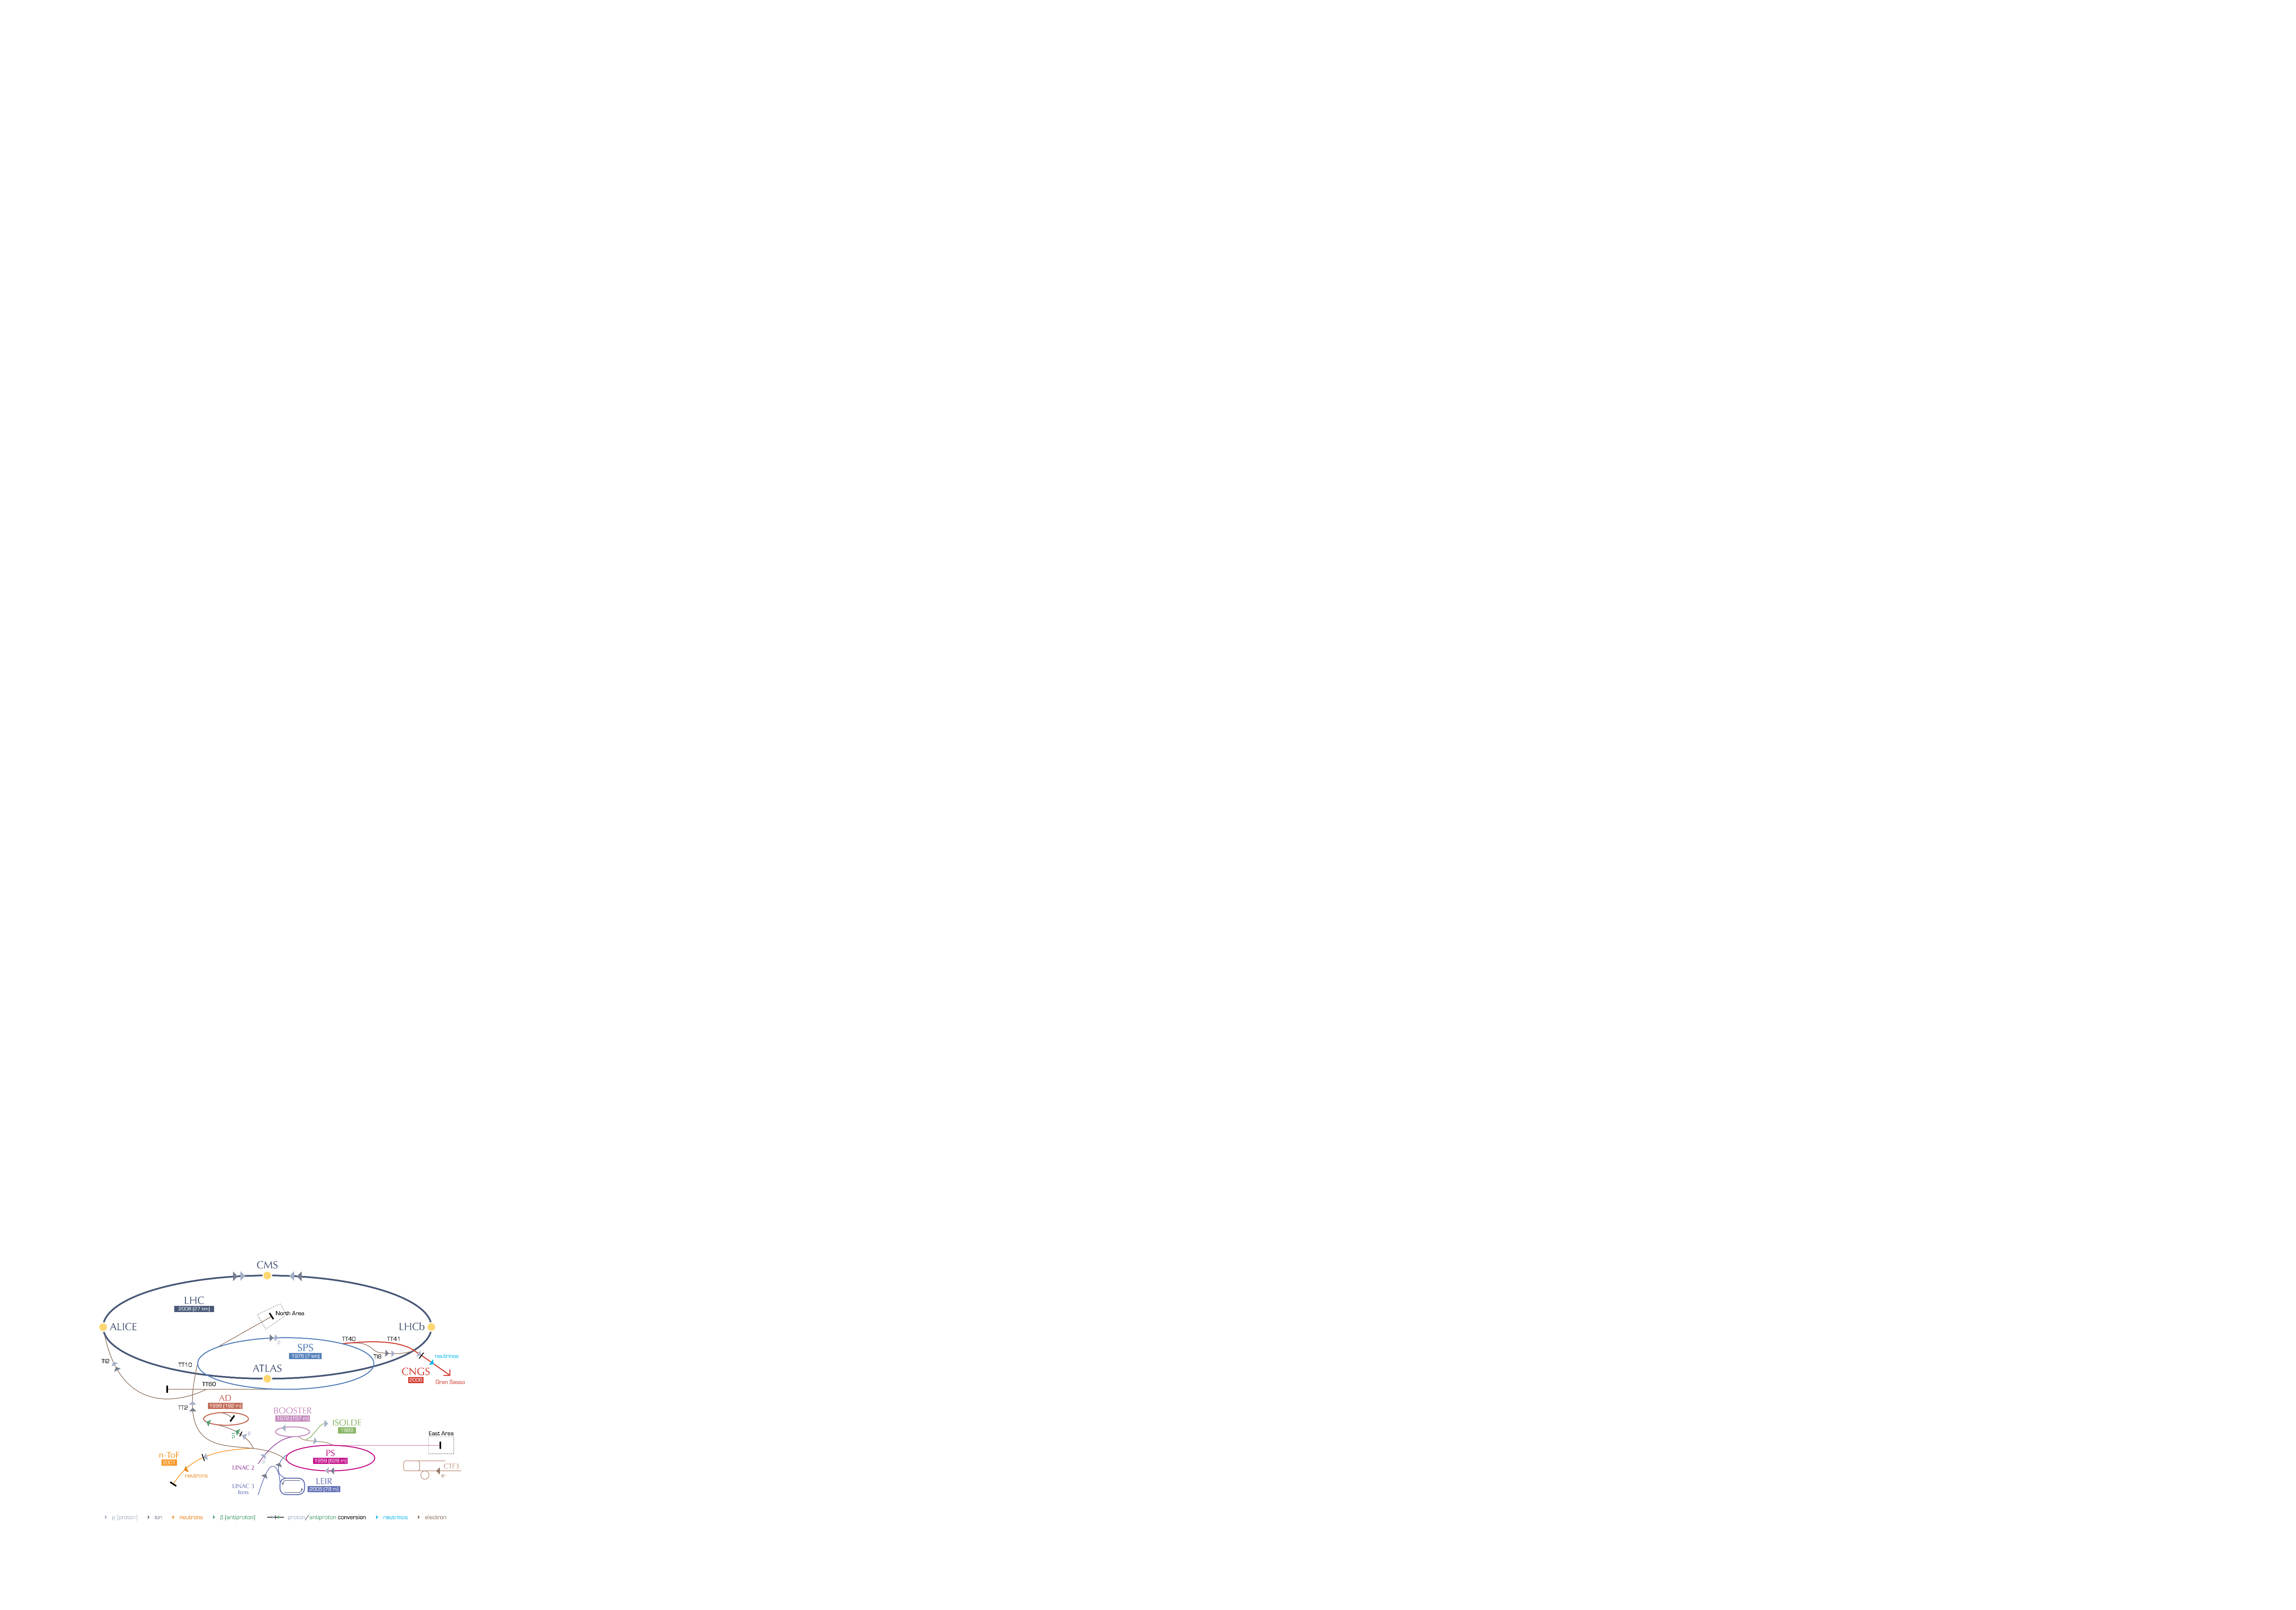
\includegraphics[width=1.0\textwidth]{figs/Detector/Acc_complex.pdf}
    \caption{The accelerator complex at \cern taken from Ref...}
    \label{fig:Dec_Acc_Complex}   
\end{figure}
%%%%%%%%%%%%%%%%%%%%%%%%%%%%%%%%%%%%%%%%%%%%%%%%%%%%%%%%%%

In addition to protons, the complex can accelerate other ions including lead, and more recently, argon and xenon {\color{Red}cite}. These start in a dedicated linear accelerator, LINAC3, where the electrons are stripped off the ions to produce bare nuclei before being injected into the Low Energy Ion Ring (LEIR). This ring raises the ion's energy from 4.2\mev to 72\mev. 

Either protons or ions can then be injected in the Proton Synchrotron (PS), \cern's first synchrotron. Once the world's highest energy particle accelerator, this now accelerates the particles up to 25\gev ready to be injected into the Super Proton Synchrotron (SPS).
The SPS is the second largest accelerator at \cern, with a circumference of 7\km. It was switched on in 1976 and resulted in the notable discoveries of the \W and \Z bosons. Here, the particles are finally accelerated up to an energy of 450\gev, ready for injection into the \lhc. The particles are transferred from the SPS to the \lhc via two lines, one for each of the \lhc beam directions. The two beams, referred to as Beam 1 and Beam 2, travel clockwise and anti-clockwise respectively when viewed from above.

The particles travel through the accelerator complex in groups called bunches. These typically contain around $10^{11}$ protons and are necessary as a result of the Radio-frequency (RF) cavities that accelerate the particles. The bunches are sequentially transferred between the accelerators in collections called trains. The bunch-trains are transferred from the SPS to the \lhc in a series of injections. Although the \lhc has a capacity for 3465 bunches, the nominal operating conditions has only 2808 of these spaces filled. This leaves enough for room magnets that redirect the beams to turn on and off between the bunches so as not to damage the instrumentation around the beam-pipes.  

Once the \lhc is at capacity the beams are accelerated from the injection energy of 450\gev to the nominal energy of up to 7\tev. This is achieved using eight RF cavities per beam to increase the energy and 1232 superconducting dipole magnets that bend the trajectory of the charged particles, ensuring they follow the paths dictated by the circular tunnels. The 15\m long dipole magnets contain superconducting niobium-titanium cables, kept cool at 1.9\,K using super-fluid helium. The 11,850\,A current that flows through the magnets generates a large magnetic field of 8.33\,T. The current is gradually and synchronously ramped as the particles are accelerated, such that the same trajectory is maintained. 

The \lhc contains a wealth of other magnets, another 8,361 in addition to the dipole magnets, that optimise the orbit of the beams. This includes ensuring the beams remain tightly packed together, as well as many higher order corrections.   

During the injection and acceleration of the beams no collisions take place. Once the beams are at the nominal energy and beam profiles have been optimised the two beams are brought together at four interaction points around the rings. Magnets are used to both move the beams such that they crossover and to squeeze the beams to a smaller cross-section at the collision points, increasing the likelihood of collisions.    

{\color{Red}
\begin{itemize}
\item Brief overview of the life of a proton from source to \lhc
\item injection points
\item Phases of \lhc?
\end{itemize}
}
A total of seven experiments are located at the \lhc, situated in four caverns. The four largest are \atlas, \cms, \lhcb and \alice. The TOTEM, LHCf and MoDEL experiments are located in the same caverns as \cms, \atlas and \lhcb respectively. 



\subsection{The \lhcb collaboration} 

The \lhcb collaboration is made up of around 800 scientists from 72 different institutions in 16 countries. The primary physics goals of the collaboration include
\begin{itemize}
\item searching for indirect signs of new physics from \CP violation
\item searching for rare decays of \bquark- and \cquark-hadrons. 
\end{itemize}  



\subsection{Beam conditions at \lhcb}
{\color{Red}
\begin{itemize}
\item \lhc optics
\item crossing angle
\item Luminosity levelling
\end{itemize}
}


\section{The \lhcb detector}

This section provides an overview of the experimental apparatus used to obtain the data analysed in this thesis.
The \lhcb detector is comprised of distinct sub-detectors, each with a dedicated purpose. These help to characterise the sub-atomic particles created in the proton-proton collisions, and enable measurements of their kinematics, trajectories and species.
This overview includes a description of the sub-detector's construction, components and performance. 

The \lhcb detector is found at Point 8 of the \lhc ring, a cavern originally built for the {\color{Red}\delphi} detector during the \lep era. A schematic representing the key components of the \lhcb detector is shown in Fig.~\ref{fig:Dec_lhcb_Schematic}. This figure displays the axes convention adopted by \lhcb, and used henceforth. The horizontal axis is labelled the $z$-axis and is parallel to the direction of the beams. The figure's vertical axis is the $y$-axis, increasing as one moves from the cavern up to ground level. The $x$-axis is in the dimension perpendicular to the plane of the figure. The $x$-axis increases as one moves towards the centre of the \lhc ring. The counter-rotating beams of protons are collided at the far left of this figure, at the origins of the $y$- and $z$-axes.   

%%%%%%%%%%%%%%%%%%%%%%%%%%%%%%%%%%%%%%%%%%%%%%%%%%%%%%%%%%
\begin{figure}[!h]
    \centering
    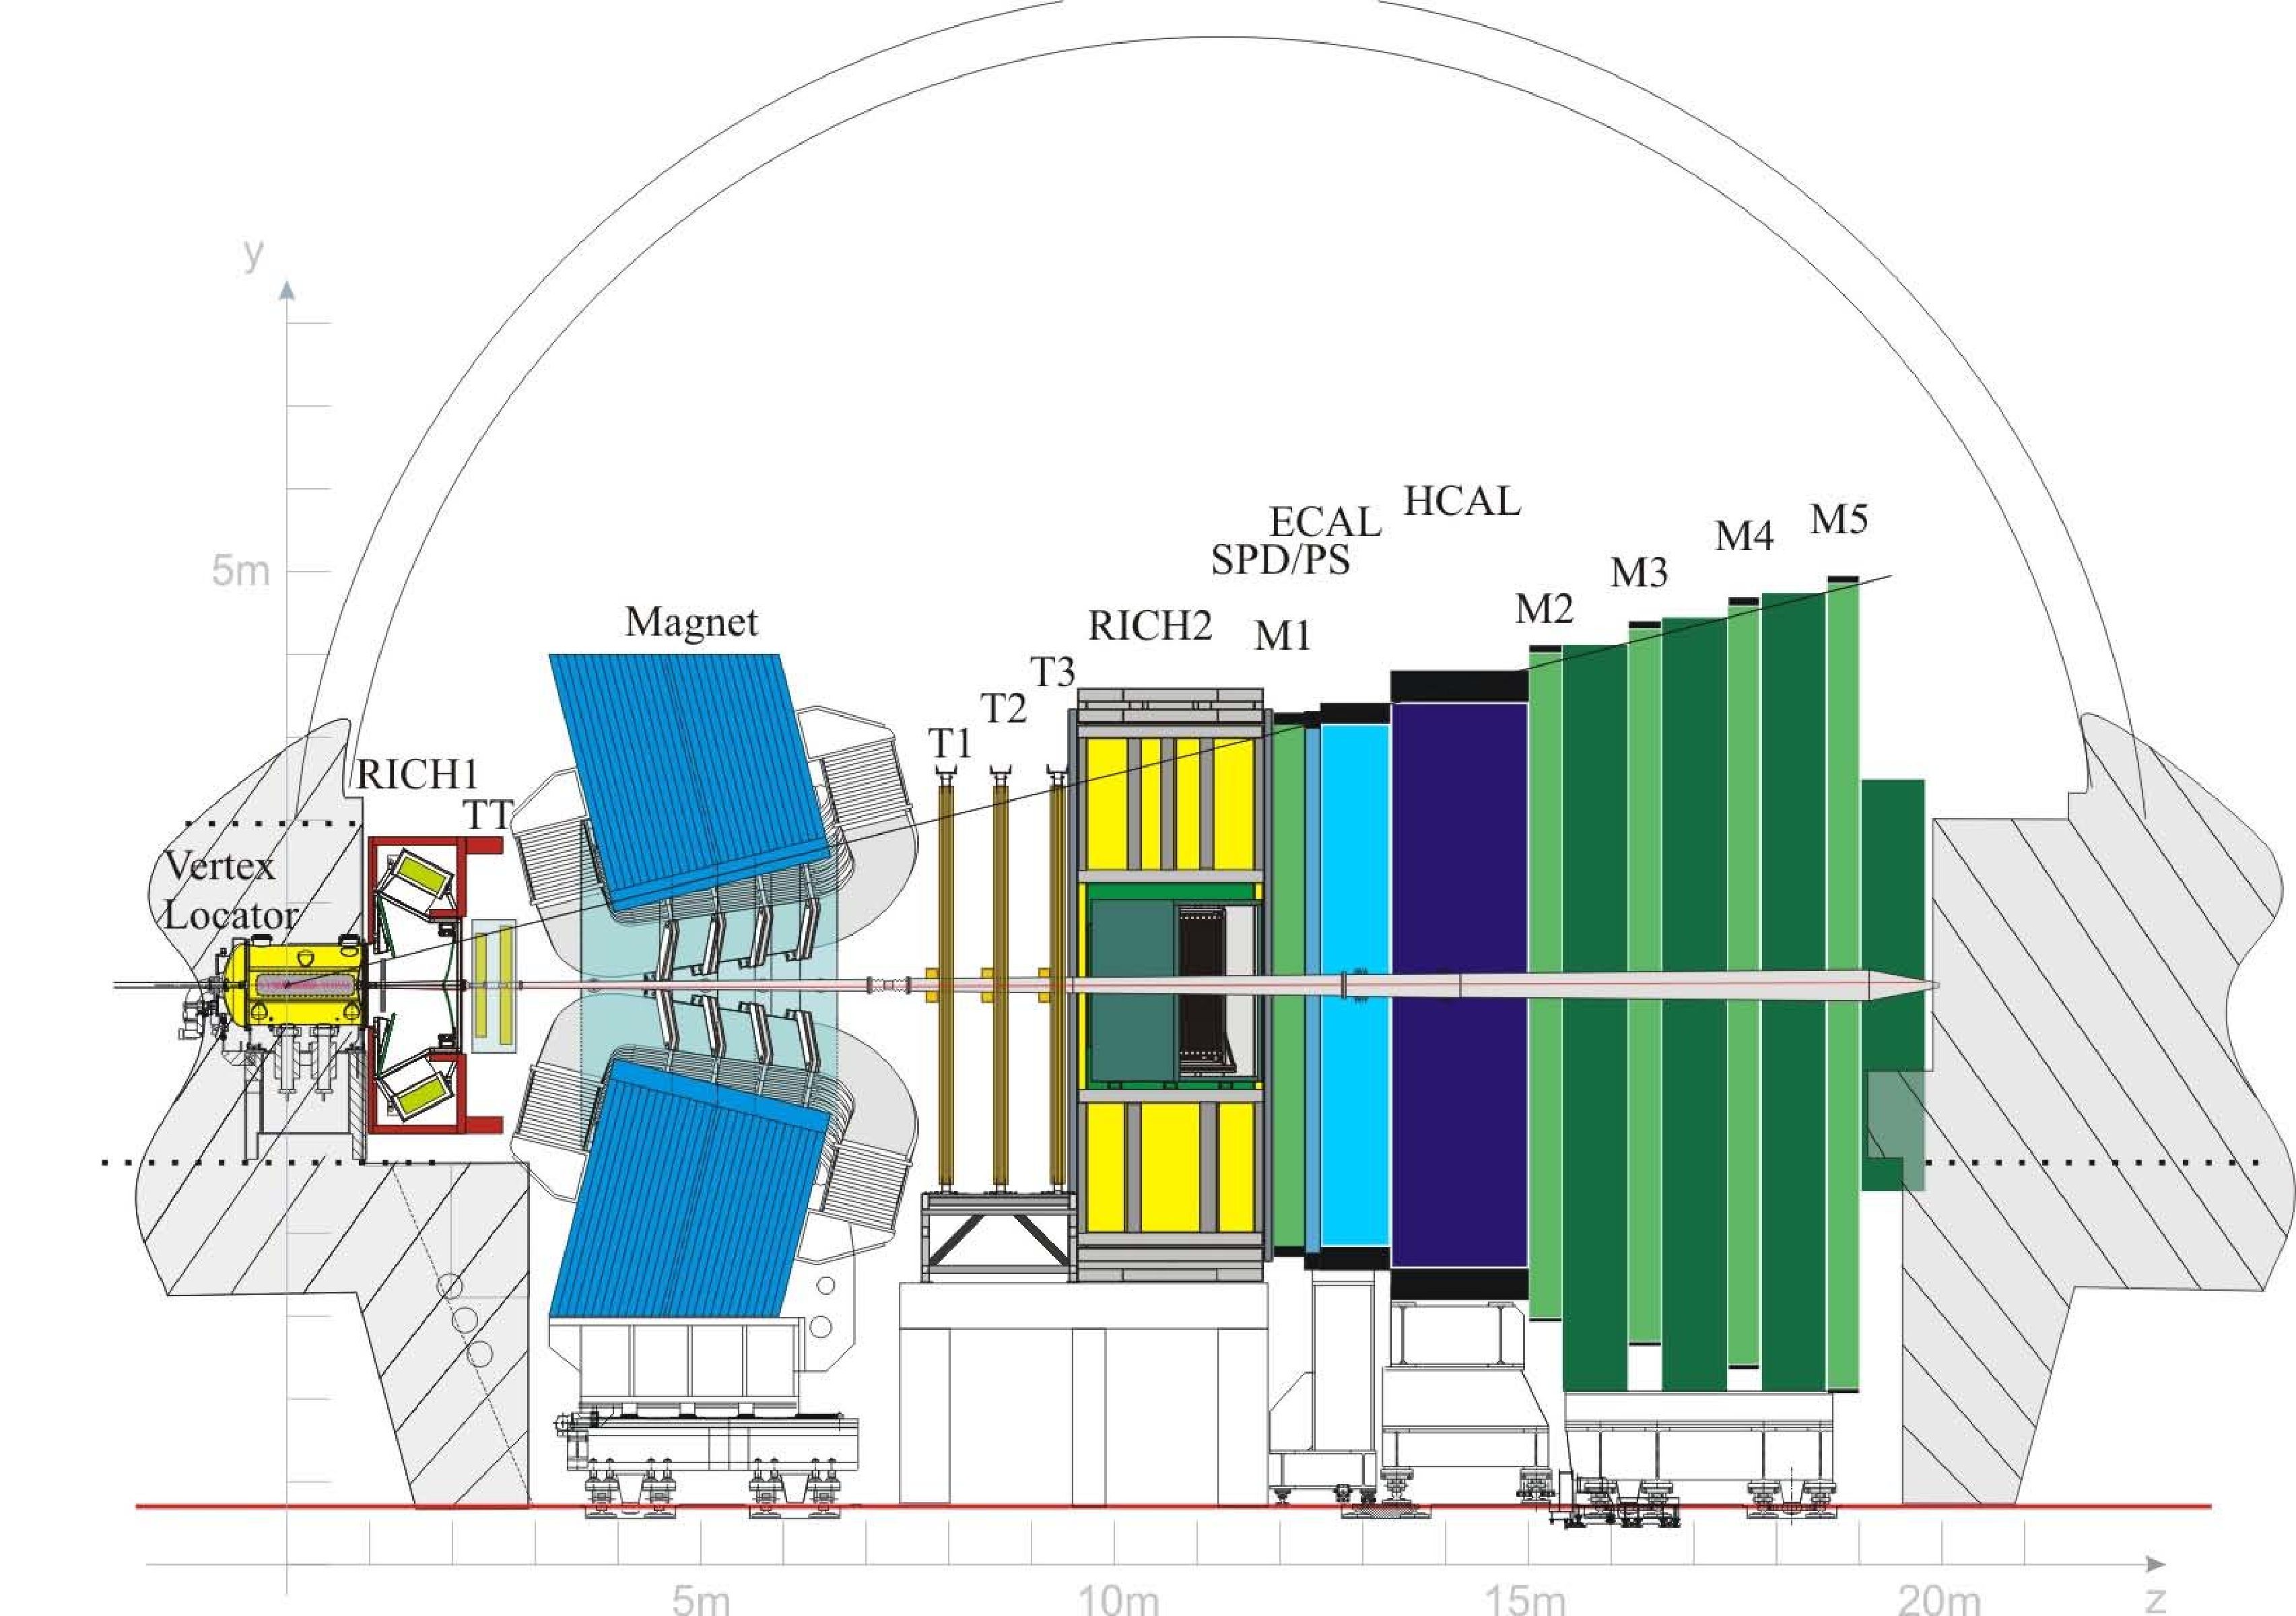
\includegraphics[width=0.8\textwidth]{figs/Detector/LHCb_Detector_Schematic.pdf}
    \caption{Schematic of the \lhcb detector, from Ref.~\cite{Alves:2008zz}.}
    \label{fig:Dec_lhcb_Schematic}   
\end{figure}
%%%%%%%%%%%%%%%%%%%%%%%%%%%%%%%%%%%%%%%%%%%%%%%%%%%%%%%%%%



Running along the centre of the detector is the \lhcb beampipe. The primary role is to separate the inner vacuum chamber from the rest of the cavern, allowing the beams to proceed unimpeded by the air. The majority of the beampipe is made of beryllium, with smaller sections made out of aluminium alloys or stainless steel. Although beryllium is a highly toxic and fragile material it has a long radiation length, allowing the incident particles to traverse the pipe walls with minimal interactions.  


{\color{Green}
\begin{itemize}
\item Distribution of bb pairs
\end{itemize}
}

\subsection{Magnet}

The \lhcb detector contains a warm dipole magnet that bends the trajectories of charges particles, allowing measurements of the particles' momentum. The magnet has two saddle-shaped coils inside a square yoke that generate an integrated magnetic field of 4 Tm.  
The magnetic field is aligned along the $y$-axis, bending the charged particles in the horizontal plane. The polarity of the magnetic is routinely switched during data taking. This helps to understand and cancel systematic effects that may affect measurements of \CP asymmetries. The two magnet polarities are referred to \emph{MagDown} and \emph{MagUp}, corresponding to a field in the negative and positive $y$-axis direction respectively.   

A schematic of the magnet is shown in Fig.~\ref{fig:Dec_magnet}, along with the strength of the magnetic field as a function of the $z$-axis position. Both magnet polarities are represented in this figure. 

{\color{Red}
\begin{itemize}
\item Magnet: purpose and design 
\end{itemize}
}


%%%%%%%%%%%%%%%%%%%%%%%%%%%%%%%%%%%%%%%%%%%%%%%%%%%%%%%%%%
\begin{figure}[!h]
    \centering
    \begin{subfigure}[t]{0.4\textwidth}
        \centering
        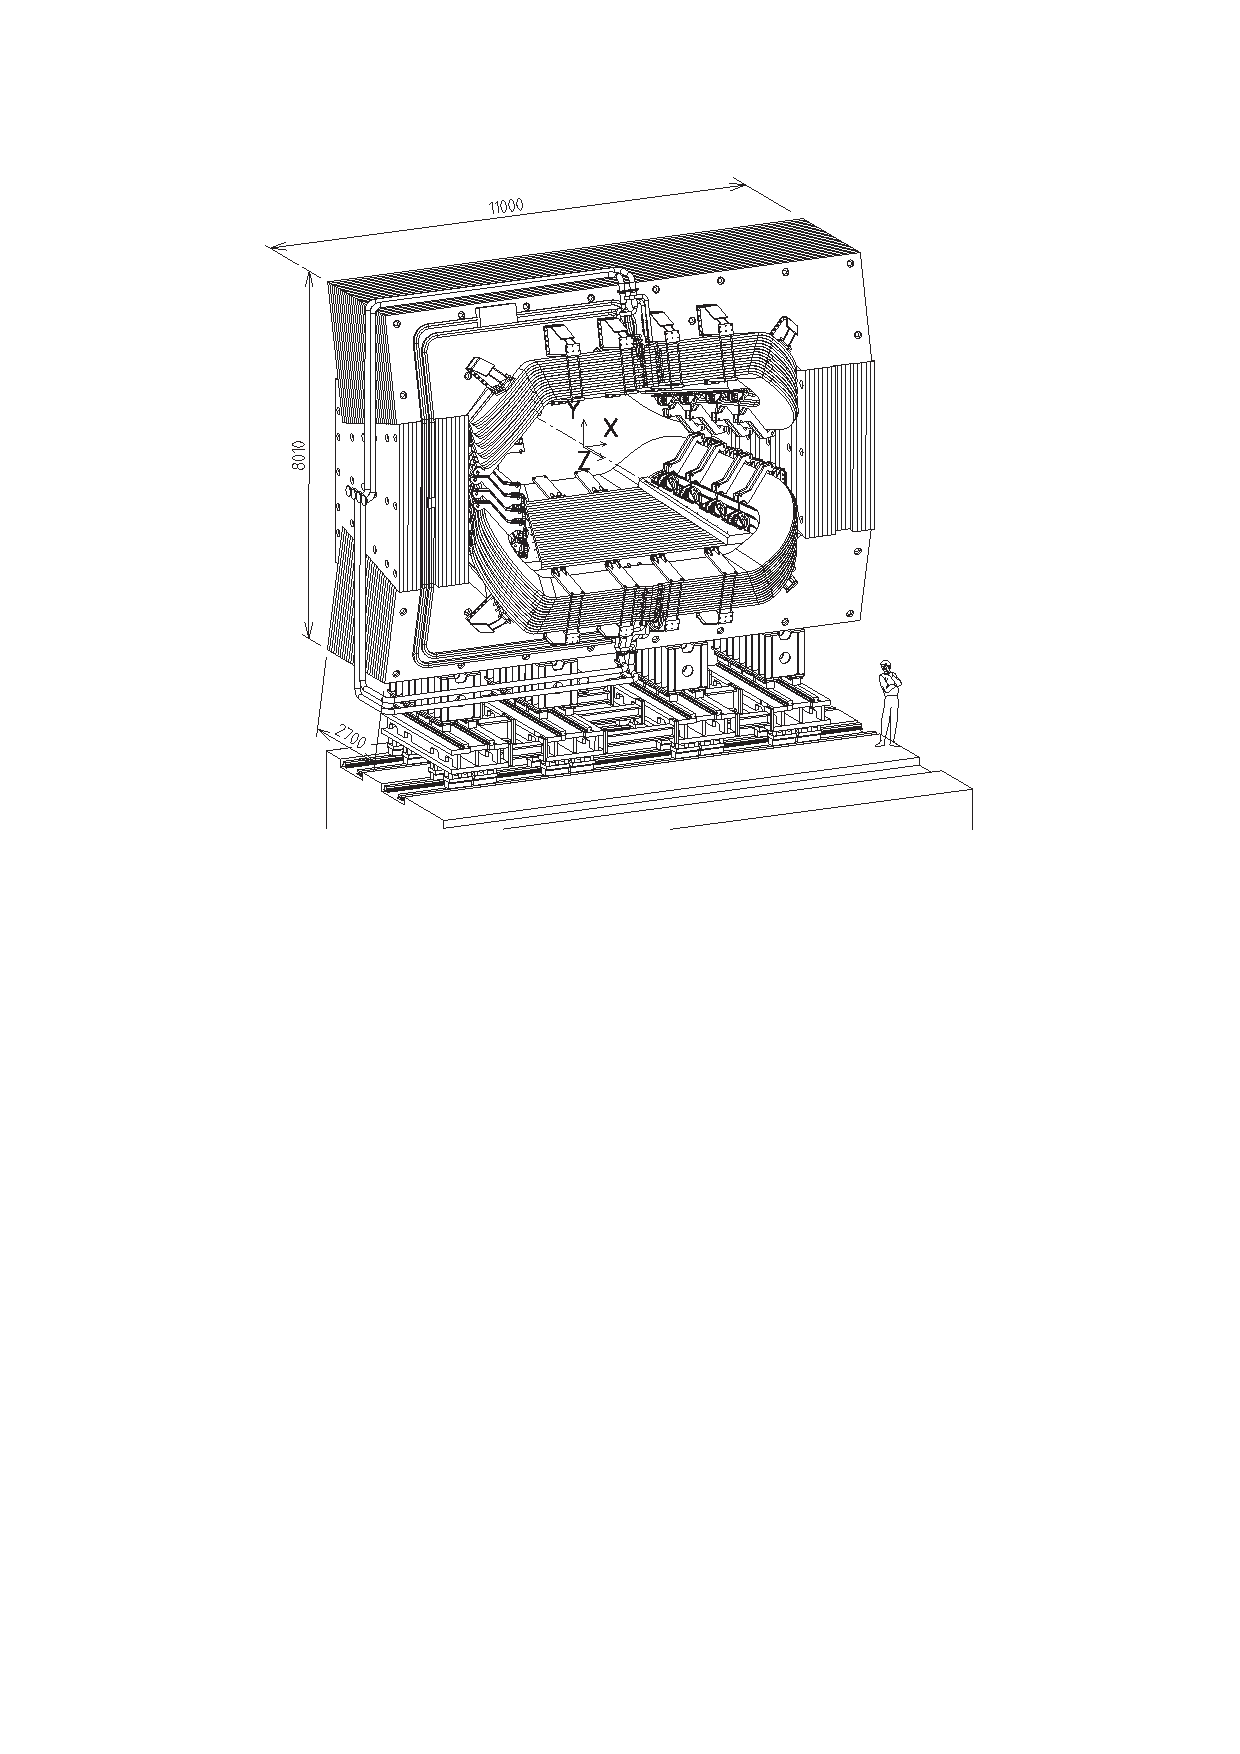
\includegraphics[width=1.0\textwidth]{figs/Detector/magnet_schematic.pdf}
    \end{subfigure}
    \begin{subfigure}[t]{0.4\textwidth}
        \centering
        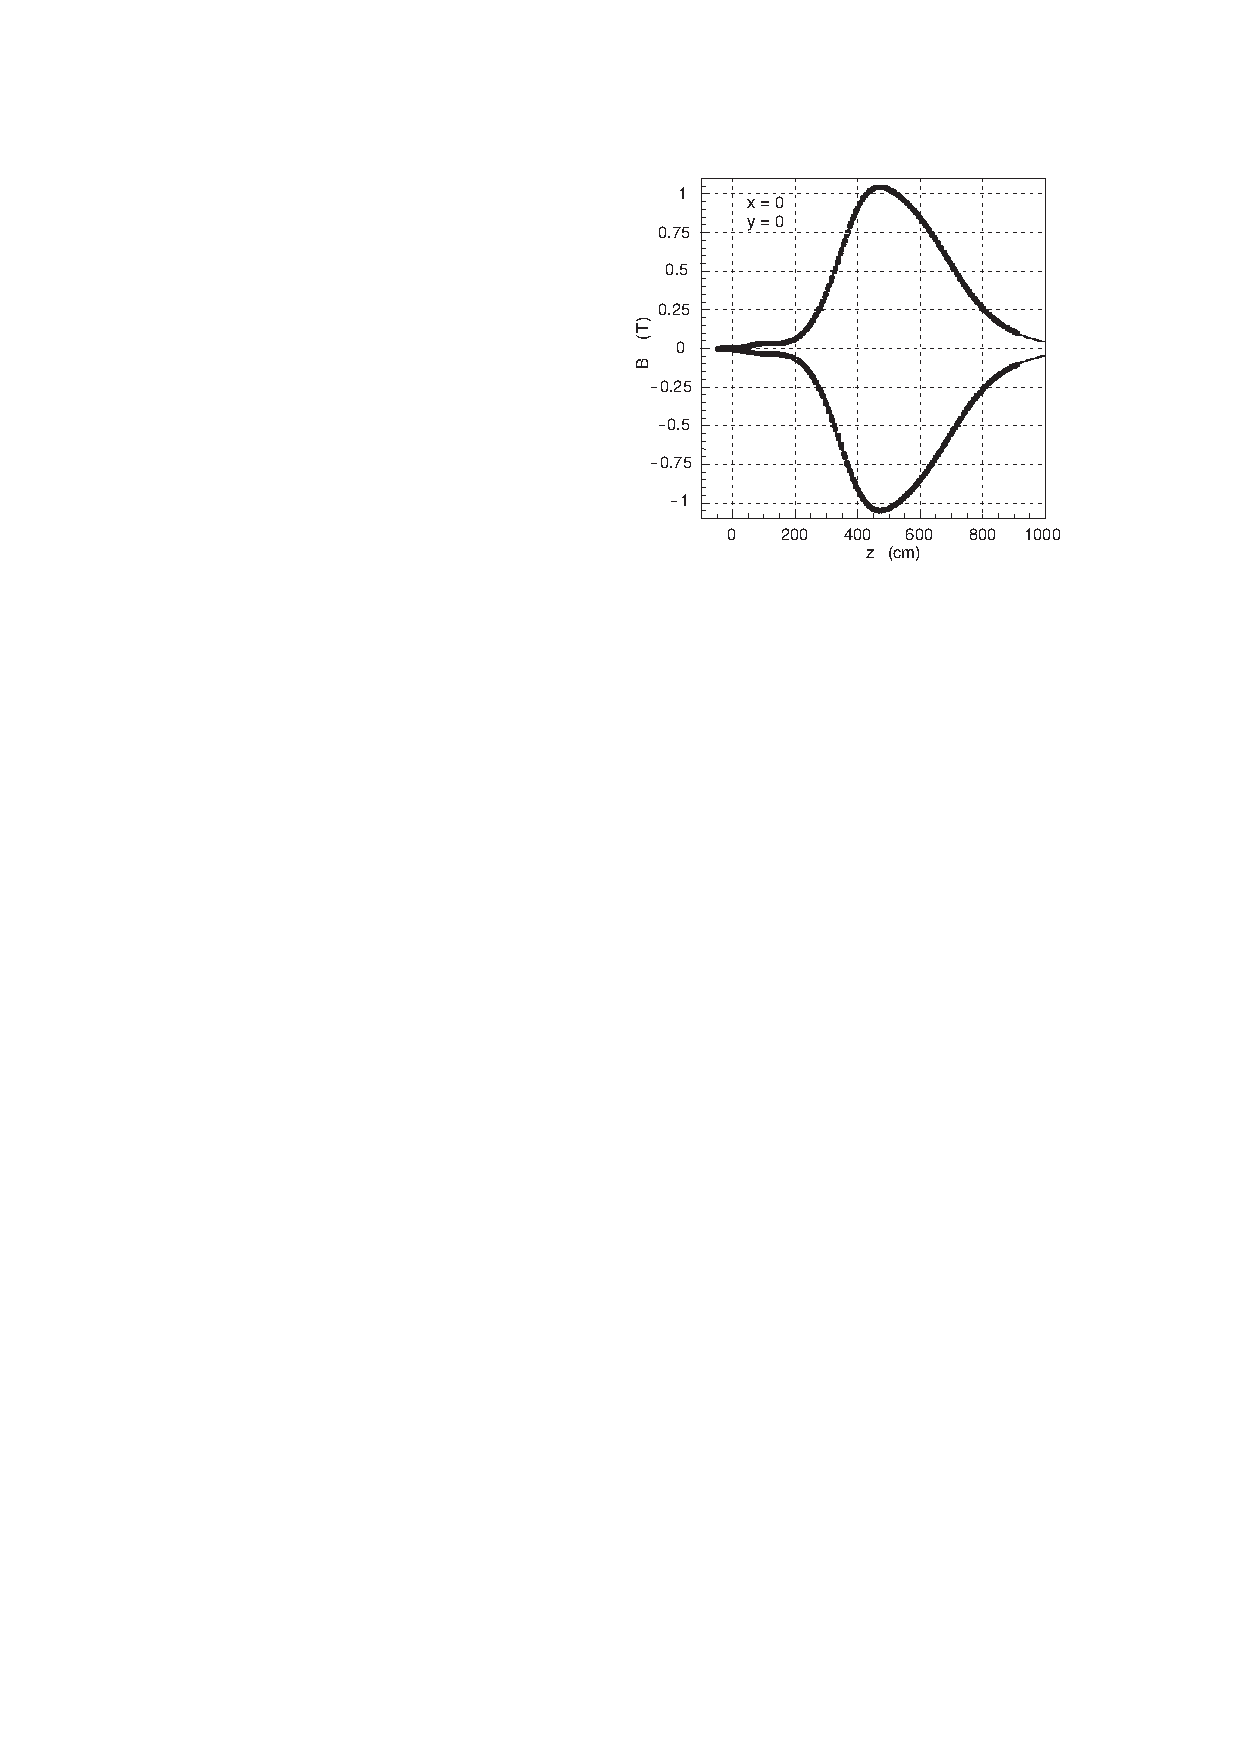
\includegraphics[width=1.0\textwidth]{figs/Detector/magnet_B_field.pdf}
    \end{subfigure}
    \caption{Schematic of the \lhcb warm dipole magnet (left) and the magnetic field strength along the $z$-axis (right) from Ref.~\cite{Alves:2008zz}.}
    \label{fig:Dec_magnet}   
\end{figure}
%%%%%%%%%%%%%%%%%%%%%%%%%%%%%%%%%%%%%%%%%%%%%%%%%%%%%%%%%%


\subsection{Vertex Locator}

The first sub-detector to make measurements of the particles produced in proton-proton collisions is the Vertex Locator (\velo) encompassing the collision region. This sub-detector make precise measurements of the track positions of charged particles as they emanate out of the collisions. A high level of precision is required to identify the secondary vertices characteristic of \bquark- and \cquark-hadron decays. These secondary vertices are typically displaced from the interaction position as a result of the long lifetimes associated to these heavy-flavour hadrons. This is achieved by measuring the track coordinates using silicon sensors placed a close to the \lhc beam as safety allows. The \velo sensors are semicircular devices placed on either side of the beam. To allow the sensors to instrument the innermost region around the interaction point the two halves of the \velo can move horizontally in and out. During normal data taking this allows the sensors to be 7\mm away from the interaction point yet still be a safe distance away from the beams at injection. 

%%%%%%%%%%%%%%%%%%%%%%%%%%%%%%%%%%%%%%%%%%%%%%%%%%%%%%%%%%
\begin{figure}[!h]
    \centering   
    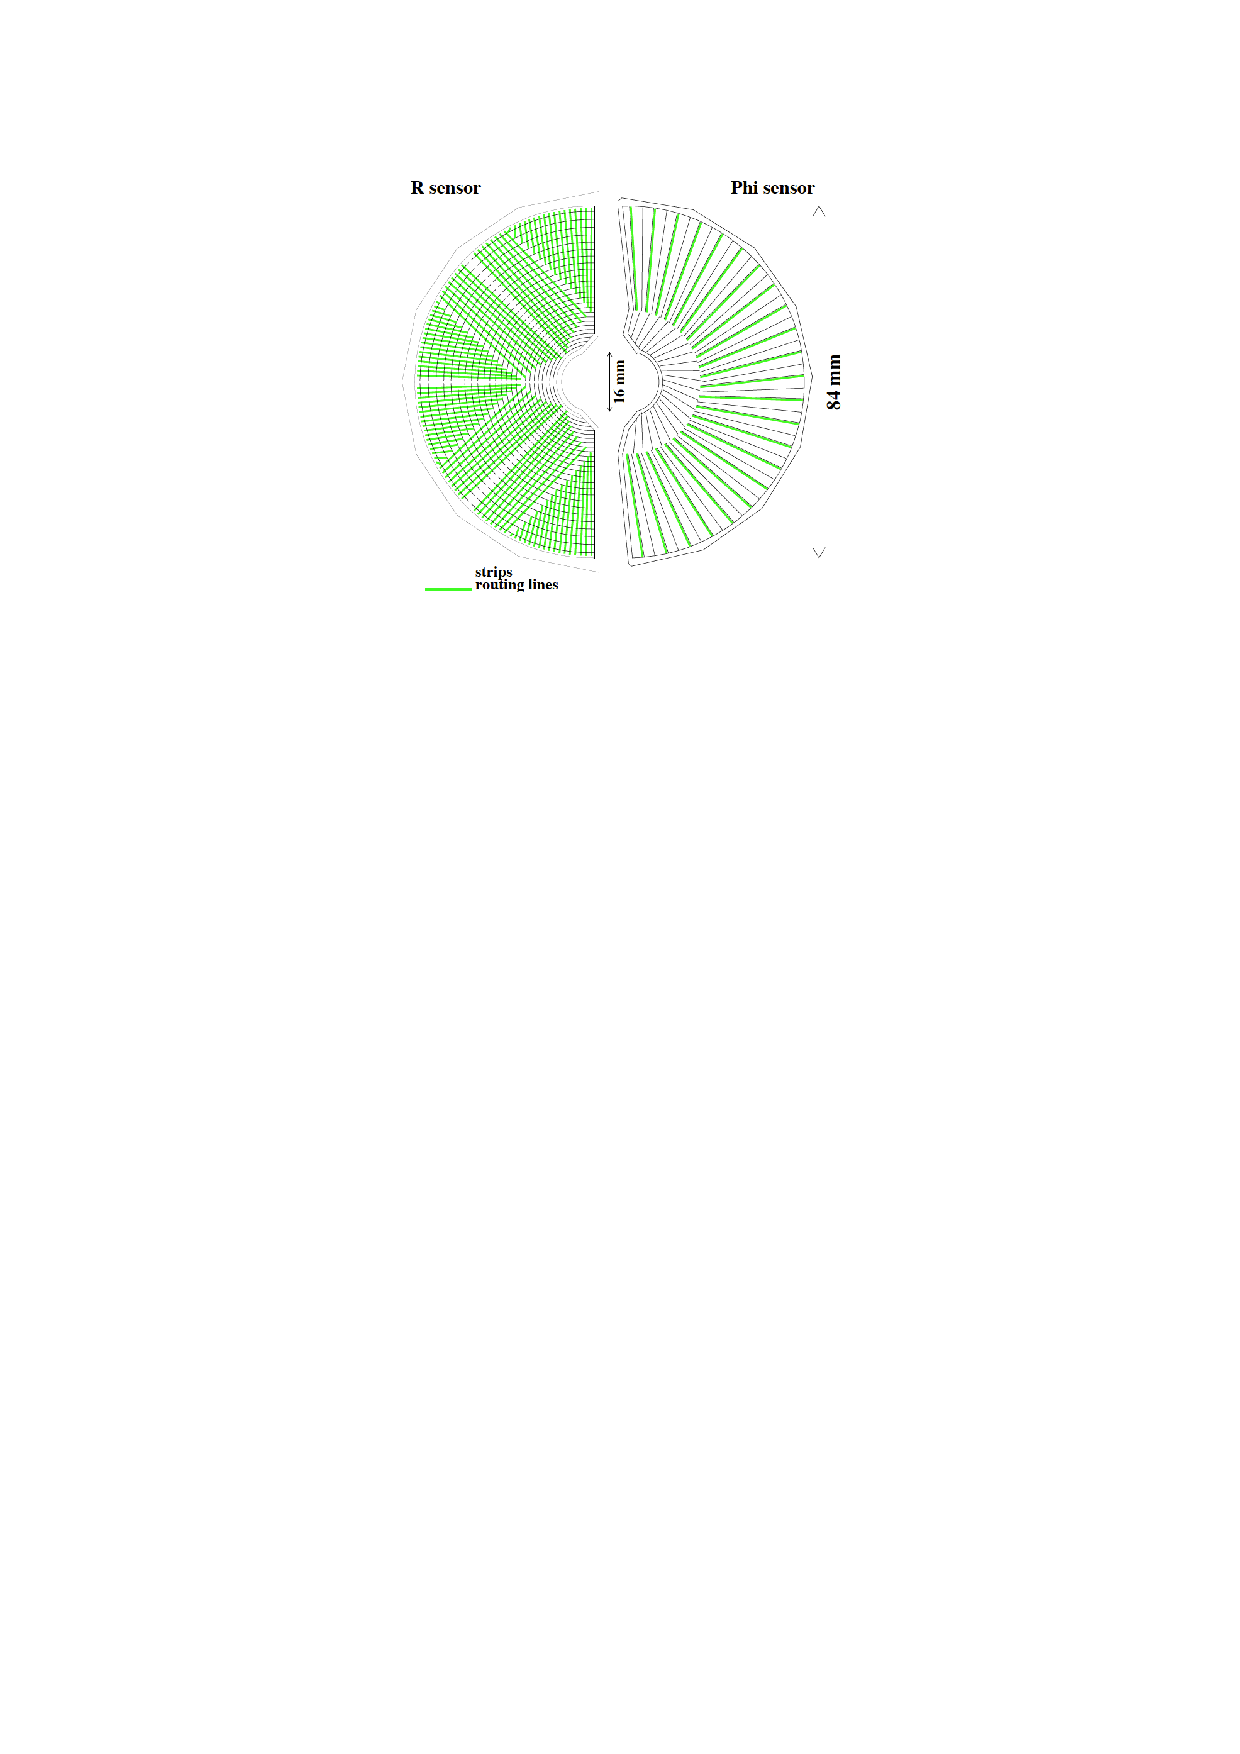
\includegraphics[width=0.4\textwidth]{figs/Detector/velo_r_phi_sensor.pdf}
    \caption{Schematic of an $r$- and $\phi$-sensor in the \velo sub-detector, from Ref.~\cite{LHCb-DP-2014-001}.}
    \label{fig:Dec_r_phi_sensor}   
\end{figure}
%%%%%%%%%%%%%%%%%%%%%%%%%%%%%%%%%%%%%%%%%%%%%%%%%%%%%%%%%%

The sensors are grouped into pairs, called modules. Each of the 21 modules on each side contains sensors for measuring the radial and azimuthal coordinates of the tracks, referred to as $r$- and $\phi$-sensors respectively. A schematic of the two sensor types is shown in Fig.~\ref{fig:Dec_r_phi_sensor}, illustrating the silicon strips and readout channels. 


The \velo modules are arranged to ensure coverage of particles emerging in forward region at angles of 15--300\mrad. The arrangement allows tracks within this acceptance to interact in at least three sensors as shown in Fig.~\ref{fig:Dec_velo_sensor_layout}.   
The modules extend both forward and backwards of the interaction region. Although momentum measurements are not possible for backward tracks, the vertexing of the primary interaction can benefit from this extra information. In the far backward region there are two additional modules, measuring only the radial coordinate. These help to identify pile-up events in which there is more than one primary vertex. 

%%%%%%%%%%%%%%%%%%%%%%%%%%%%%%%%%%%%%%%%%%%%%%%%%%%%%%%%%%
\begin{figure}[!h]
    \centering
    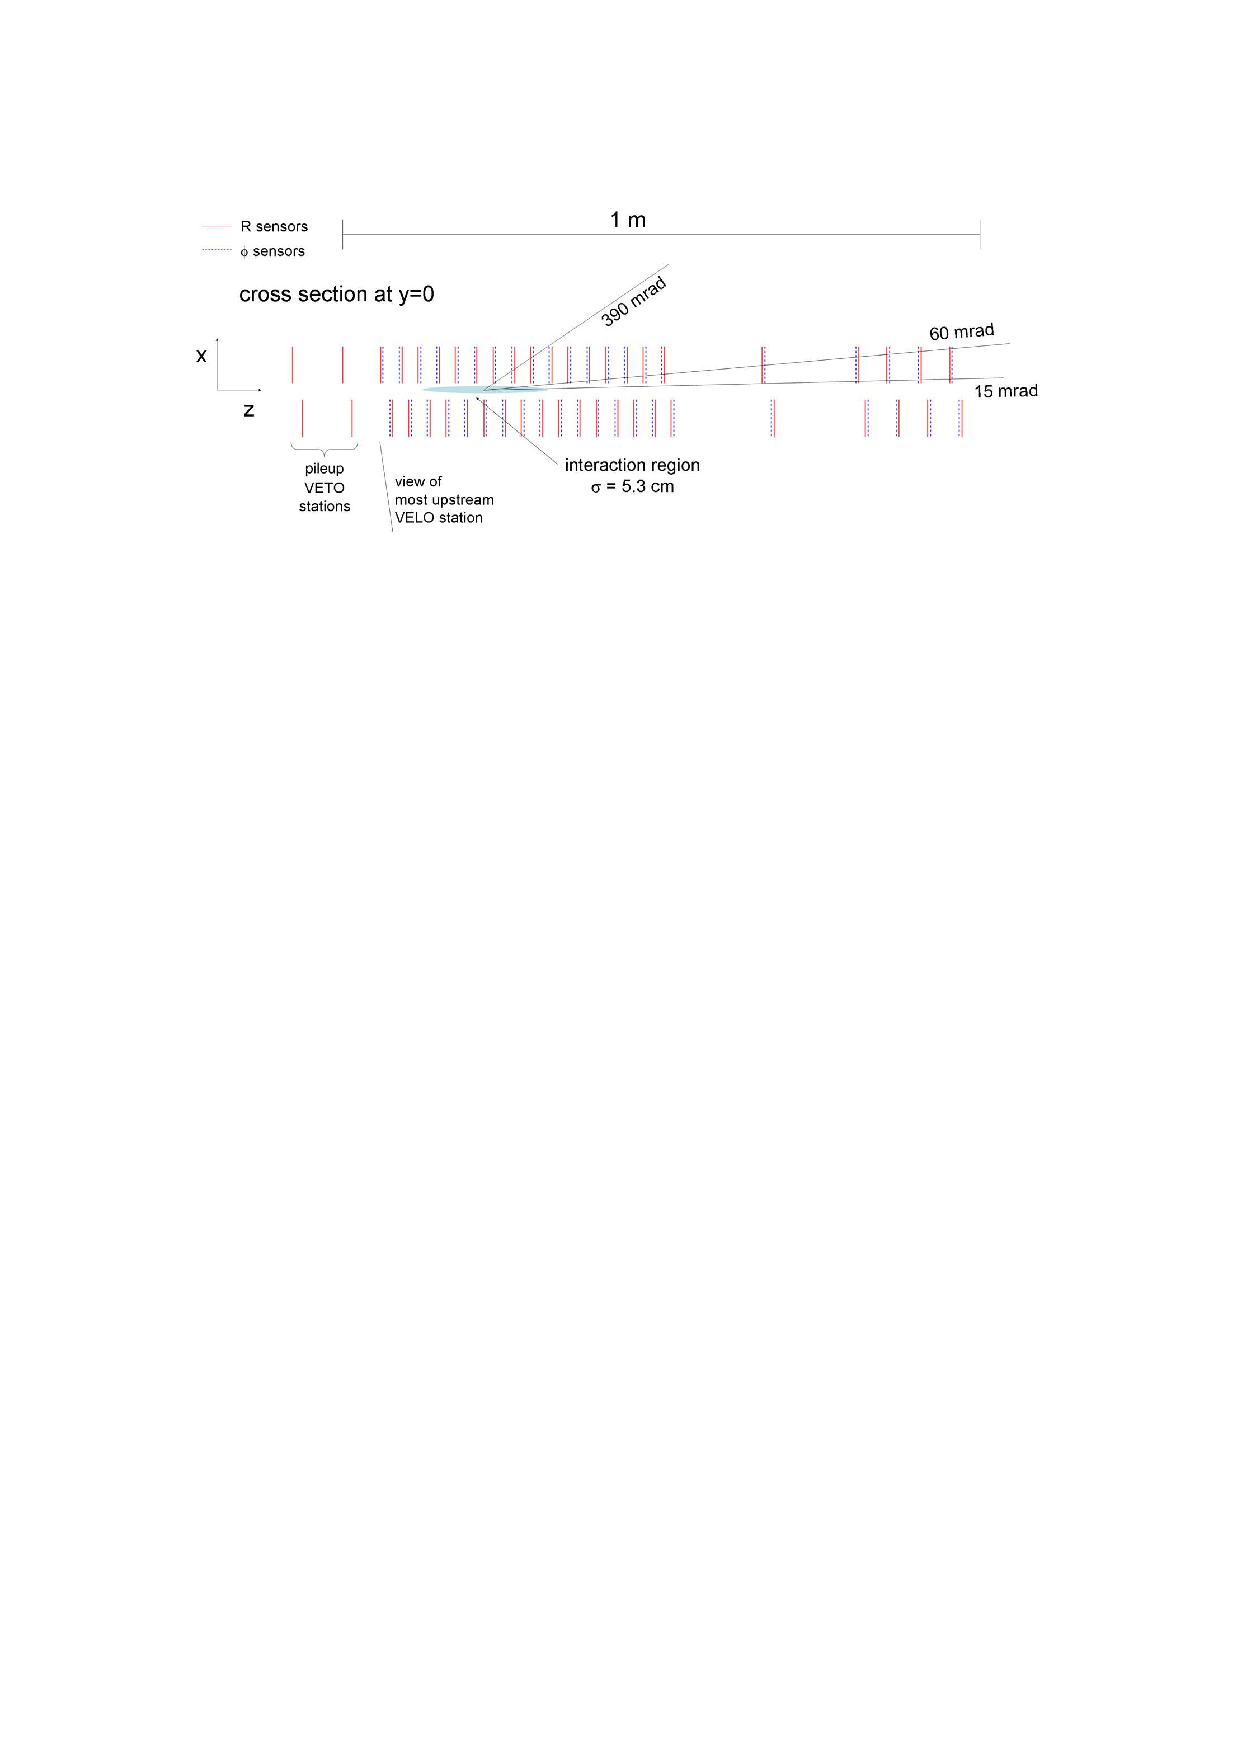
\includegraphics[width=0.8\textwidth]{figs/Detector/velo_sensor_layout.pdf}
    \caption{Schematic of the sensor layout in the \velo sub-detector, from Ref.~\cite{LHCb-DP-2014-001}.}
    \label{fig:Dec_velo_sensor_layout}   
\end{figure}
%%%%%%%%%%%%%%%%%%%%%%%%%%%%%%%%%%%%%%%%%%%%%%%%%%%%%%%%%%

The \velo sub-detector is constructed to operate in the unique environment close to the \lhc beams.

\begin{description}   
\item \textbf{Radiation resistance:} the \velo modules are subjected to extreme and varying amounts of radiation. The detector is designed to with stand three years of nominal \lhc running, using a radiation tolerant semiconductor construction. Additionally, the \velo modules are cooled to remove the heat created from the interactions. The sensors are maintained at a temperature between -10 and 0\degrees\,C with 24\,W of heat removed from each sensor.  
\item \textbf{Radio-frequency (RF) pick-up protection:} the electromagnetic fields generated by the \lhc beams could cause interference in the \velo detectors electronics. Therefore, a shield is used between the modules and the beam-pipe referred to as the RF-foil. This 0.3\mm thick foil separates the \velo and beam-pipe vacuums, providing additional protection to the conditions of the beams from the detector.
\end{description}   

The hits arising from particle interactions in the \velo sensors are extracted from the readout channels using custom analogue \beetle chips. The signals are digitised and combined into clusters in \tell1 readout boards~\cite{HAEFELI2006494}, 


{\color{Red}
\begin{itemize}
\item velo read out chain
\item performance in run1 and run2: track finding efficiency 
\end{itemize}
}




\subsection{Silicon Tracker}

In addition to the \velo, there are two more sub-detectors that utilise silicon sensors in order to determine tracking information. These are collectively referred to at the Silicon Tracker (\st), which is made up of two trackers; the Tracker Turicensis (\ttracker) and Inner Tracker (\intr). The \ttracker is located before the dipole magnet, whereas the \intr is positioned after, as show in Fig.~\ref{fig:Dec_lhcb_Schematic}. Although these two detectors are spatially separated, their common silicon mircostrip sensors and electronics warrant considering them together.

The silicon sensors are made up of single-sided $p^{+}$-on-$n$ sensors. The hits are read out via chips at the end of each module. These chips are the same custom analogue \beetle chips used in the \velo. The signals pass to into digitisers and then through optical fibres into \tell1 boards that perform clustering algorithms.
Both sub-detectors are cooled to 5\degrees{C} and their sealed containers flushed with nitrogen gas to prevent condensation.


{\color{Red}
\begin{itemize}
\item performance
\end{itemize}
}


\subsubsection{Tracker Turicensis}

The \ttracker is positioned before the dipole magnet and covers the entire \lhcb acceptance, standing 130\cm tall and 150\cm wide.
It is made up of four layers orientated at angles to one another. The first and fourth layers are parallel, with the second and third at angles -5\degrees and +5\degrees to these respectively. The first and second are separated from the third and fourth by 27\cm along the beam axis. The layout of the silicon modules in the \ttracker is shown in Fig.~\ref{fig:Dec_tt_layout}. The sensors are grouped into \emph{half-modules} that span half of the vertical height of the sub-detector. These are made up of seven silicon sensors and a readout hybrid at the outermost end. The readout electronics are positioned outside of the \lhcb acceptance, limiting the amount of multiple scattering due to interactions with the detector material. 

%%%%%%%%%%%%%%%%%%%%%%%%%%%%%%%%%%%%%%%%%%%%%%%%%%%%%%%%%%
\begin{figure}[!h]
    \centering
    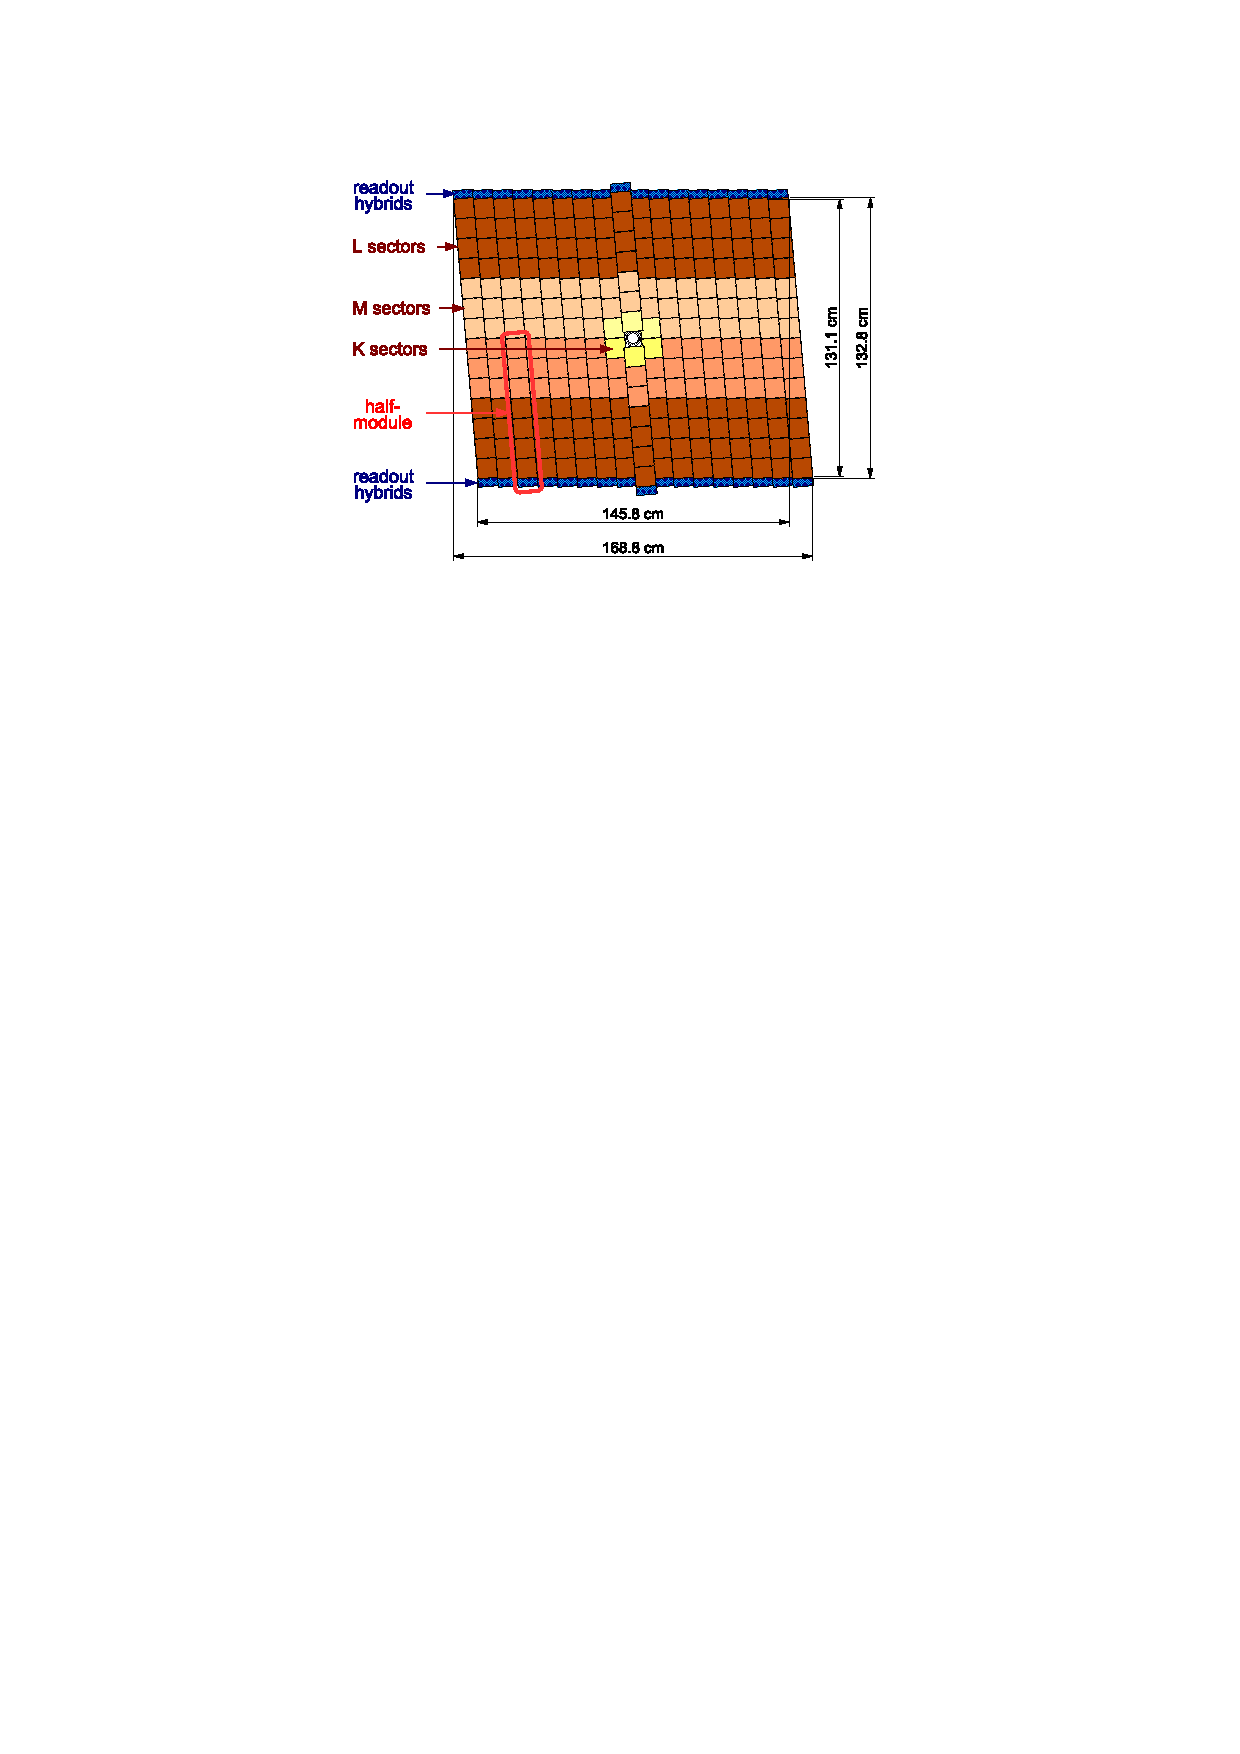
\includegraphics[width=0.6\textwidth]{figs/Detector/tt_layout.pdf}
    \caption{Schematic of the \ttracker sub-detector, from Ref.~\cite{Alves:2008zz}.}
    \label{fig:Dec_tt_layout}   
\end{figure}
%%%%%%%%%%%%%%%%%%%%%%%%%%%%%%%%%%%%%%%%%%%%%%%%%%%%%%%%%%

The \emph{half-modules} are arranged to prevent any gaps in the instrumentation. The adjacent \emph{half-modules} are offset by 1\cm along the beam axis, allowing the modules to overlap by a few millimetres in the $x$-axis. 


{\color{Red}
\begin{itemize}
\item performance
\end{itemize}
}


\subsubsection{Inner Tracker}

The \intr is the second silicon detector making up the \st. It is located after the dipole magnet in three tracking stations. As the name implies, it covers only the inner region of the acceptance, measuring 140\cm wide and 40\cm tall. The rest of the area is covered by the much larger Outer Tracker. Similar to the \ttracker, the \intr is made up of four layers positioned at slight angles to one another. However, as shown in Fig.~\ref{fig:Dec_lhcb_Schematic}, there are three separate \intr stations, each containing four layers.
These stations are constructed as of four boxes distributed around the beam-pipe in a cross shape, as shown in Fig.~\ref{fig:Dec_it_layout}. 

%%%%%%%%%%%%%%%%%%%%%%%%%%%%%%%%%%%%%%%%%%%%%%%%%%%%%%%%%%
\begin{figure}[!h]
    \centering
    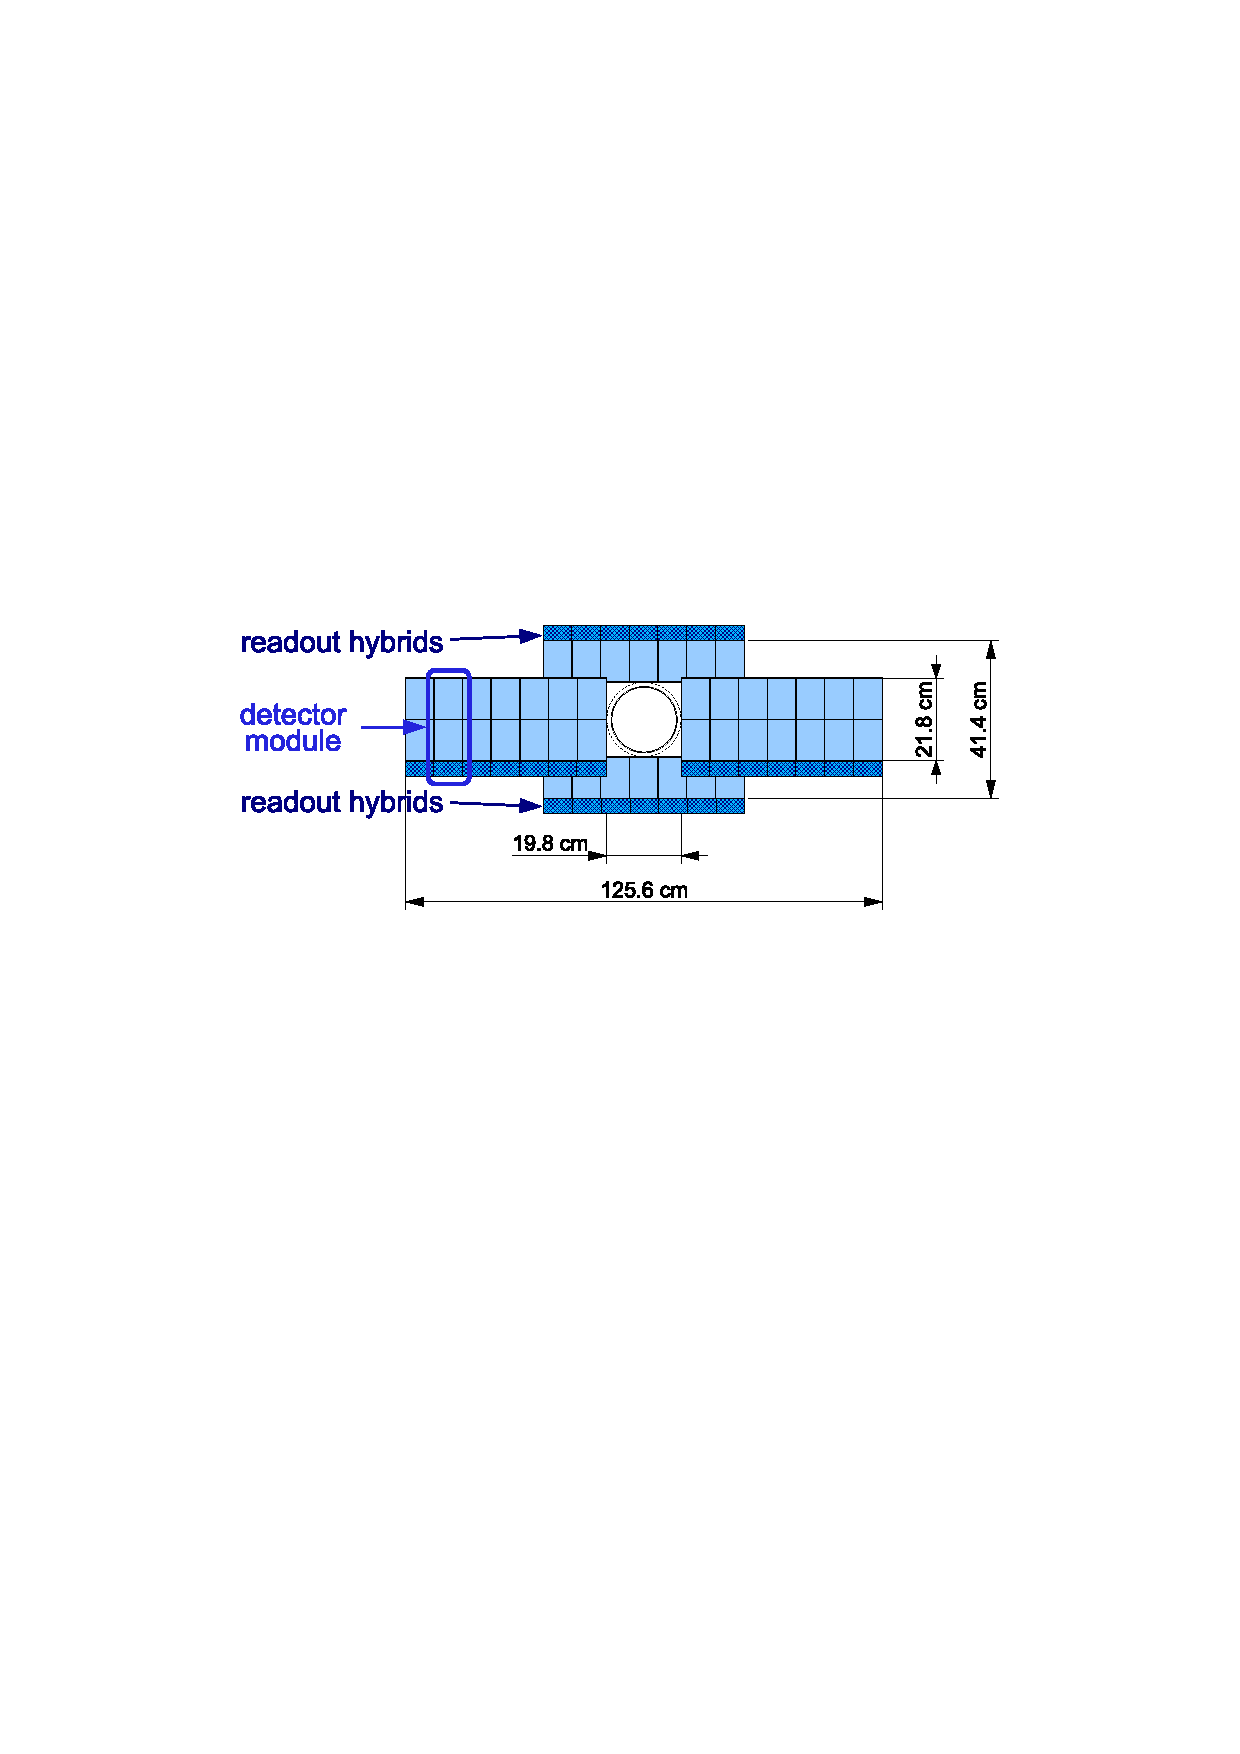
\includegraphics[width=0.6\textwidth]{figs/Detector/it_layout.pdf}
    \caption{Schematic of the \intr sub-detector, from Ref.~\cite{Alves:2008zz}.}
    \label{fig:Dec_it_layout}   
\end{figure}
%%%%%%%%%%%%%%%%%%%%%%%%%%%%%%%%%%%%%%%%%%%%%%%%%%%%%%%%%%

The detector modules consist of either one or two silicon sensors and a readout chip. These are also offset along the beam axis to allow the modules to overlap slightly in the $x$-axis.



\subsection{Outer Tracker}

In contrast to the the silicon-based sub-detectors already described, the Outer Tracker (\ot) is a straw tube tracker filled with a gaseous mixture of argon, carbon dioxide and oxygen. The 4.9\mm diameter straws are 2.4\m in length and arranged in double layers as shown in Fig.~\ref{fig:Dec_ot_schematic}. As with the \intr, the \ot is split into three stations. Each of these stations similarly has four layers arranged at angles to one another $(0\degrees,-5\degrees,+5\degrees,0\degrees)$. The arrangement of the stations and layers are also shown in Fig.~\ref{fig:Dec_ot_schematic}. The inner region occupied by the \intr is visible.
 
%%%%%%%%%%%%%%%%%%%%%%%%%%%%%%%%%%%%%%%%%%%%%%%%%%%%%%%%%%
\begin{figure}[!h]
    \centering
    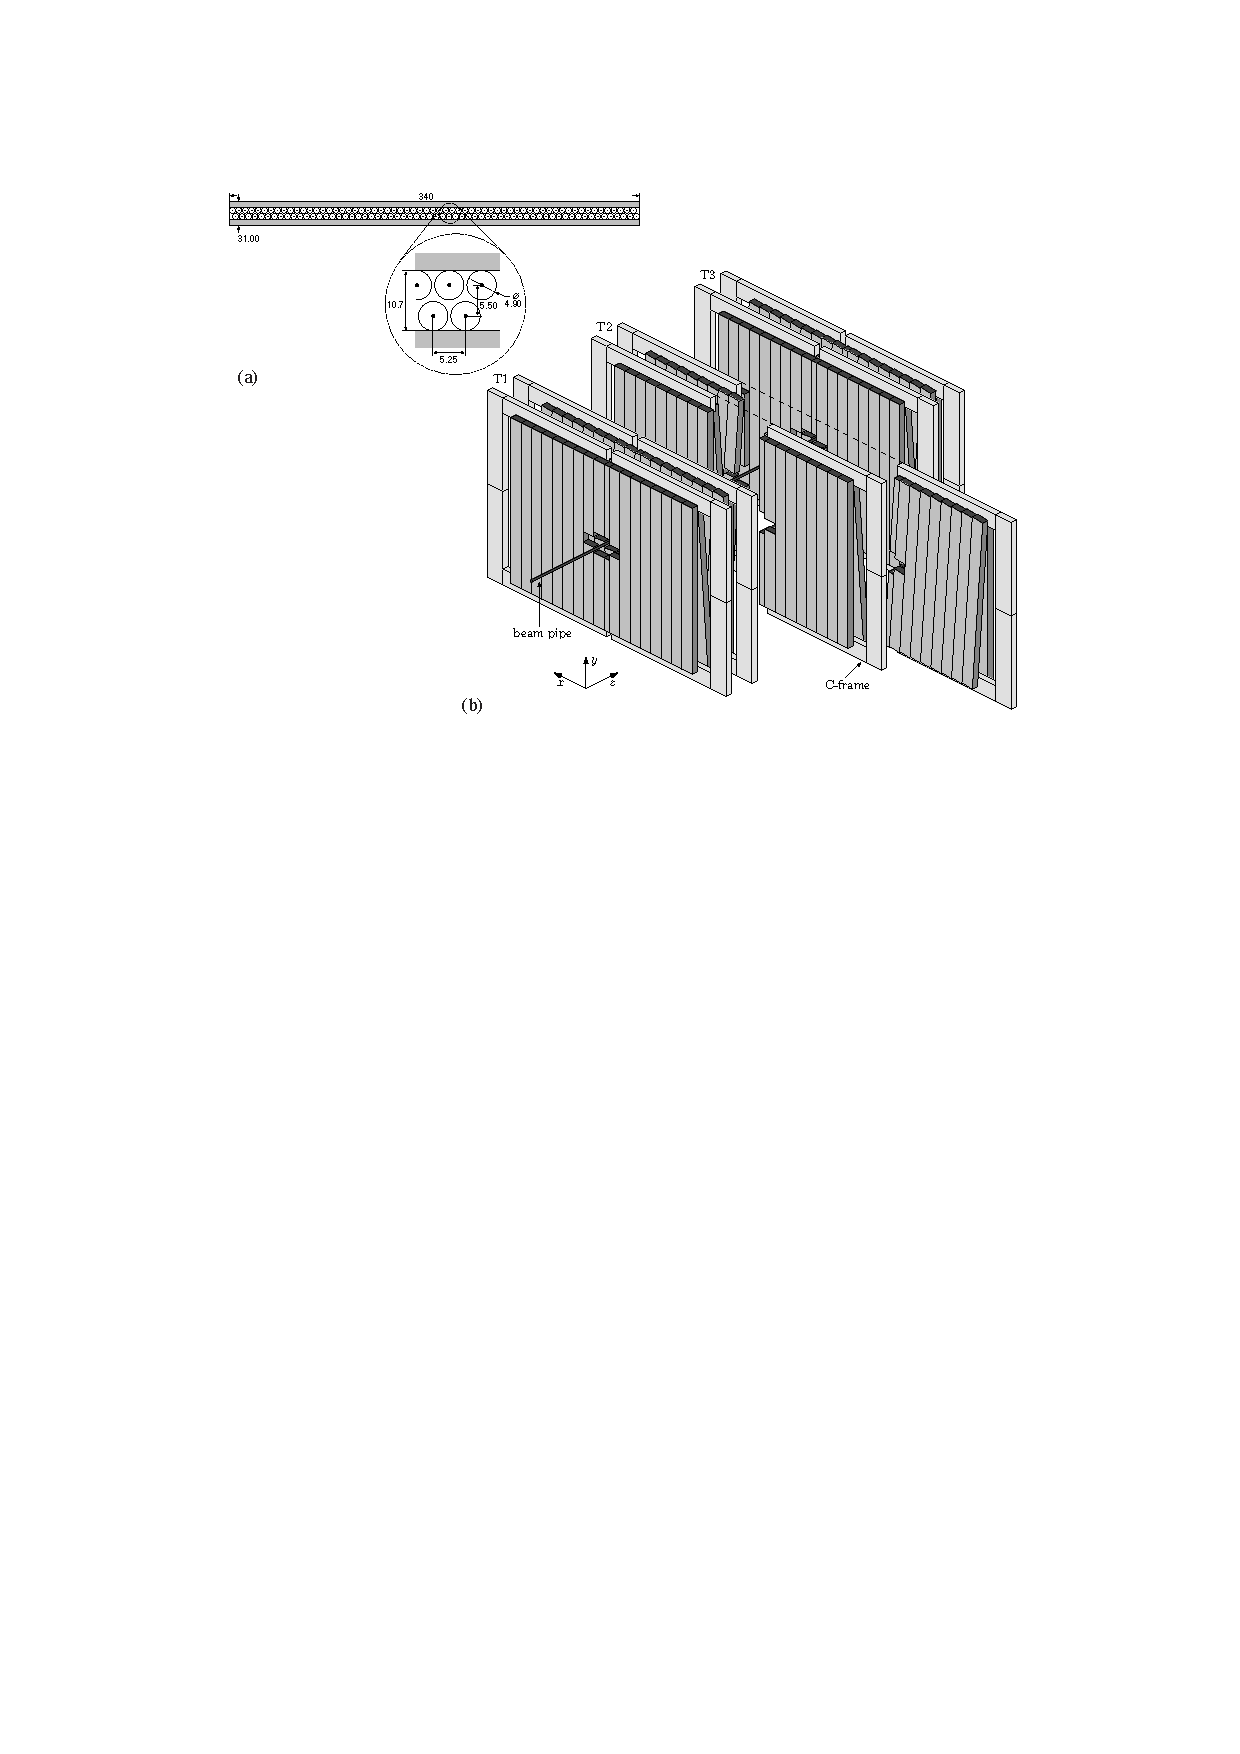
\includegraphics[width=0.8\textwidth]{figs/Detector/ot_layout.pdf}
    \caption{Schematic of the \ot sub-detector, from Ref.~\cite{LHCb-DP-2013-003}.}
    \label{fig:Dec_ot_schematic}   
\end{figure}
%%%%%%%%%%%%%%%%%%%%%%%%%%%%%%%%%%%%%%%%%%%%%%%%%%%%%%%%%%



\subsection{Ring imaging Cherenkov detectors}

The ring imaging Cherenkov detectors (\rich) provide essential information about the particle identification of tracks, allowing different species to be distinguished. This means that kaons and protons can be distinguished from the abundant pions tracks in a typical event. Two \rich sub-detectors are present, each optimised for particles with different momentums. The first, \richone, is located between the \velo and \ttracker, before the particles have passed through the magnetic field. This provides discrimination primarily for low momentum tracks between 1--60\gevc. A second sub-detector, \richtwo, is located between the \intr and \ot tracking stations and calorimeters, after the particles have travelled through the magnetic field. This caters for the higher momentum particles in the range 15--100\gevc. 


{\color{Red}
\begin{itemize}
\item rich principle 
\item mirrors
\item HPDs
\item pattern recognition 
\end{itemize}
}

%%%%%%%%%%%%%%%%%%%%%%%%%%%%%%%%%%%%%%%%%%%%%%%%%%%%%%%%%%
\begin{figure}[!h]
    \centering
    \begin{subfigure}[t]{0.4\textwidth}
        \centering        
        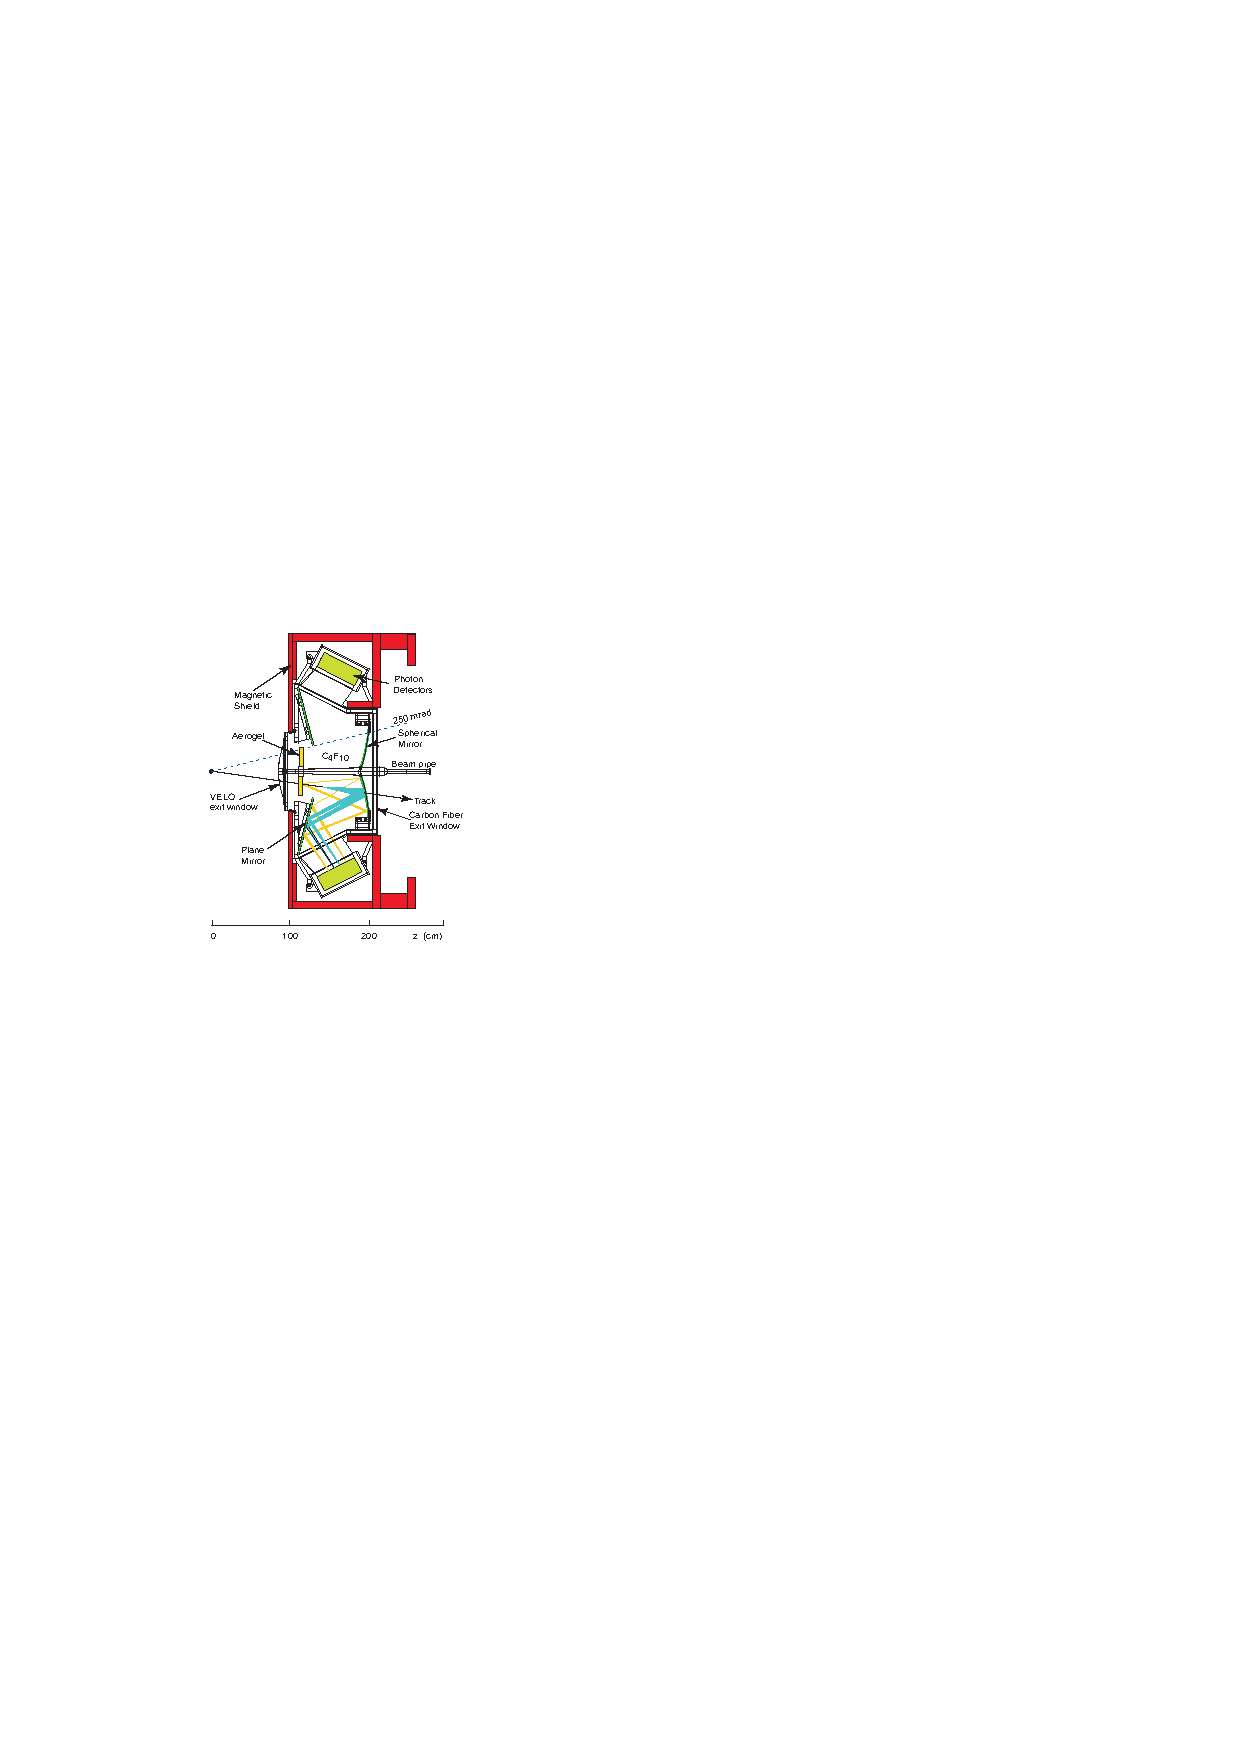
\includegraphics[width=1.0\textwidth]{figs/Detector/richone_layout.pdf}
        \caption{\richone}
    \end{subfigure}
    \begin{subfigure}[t]{0.4\textwidth}
        \centering
        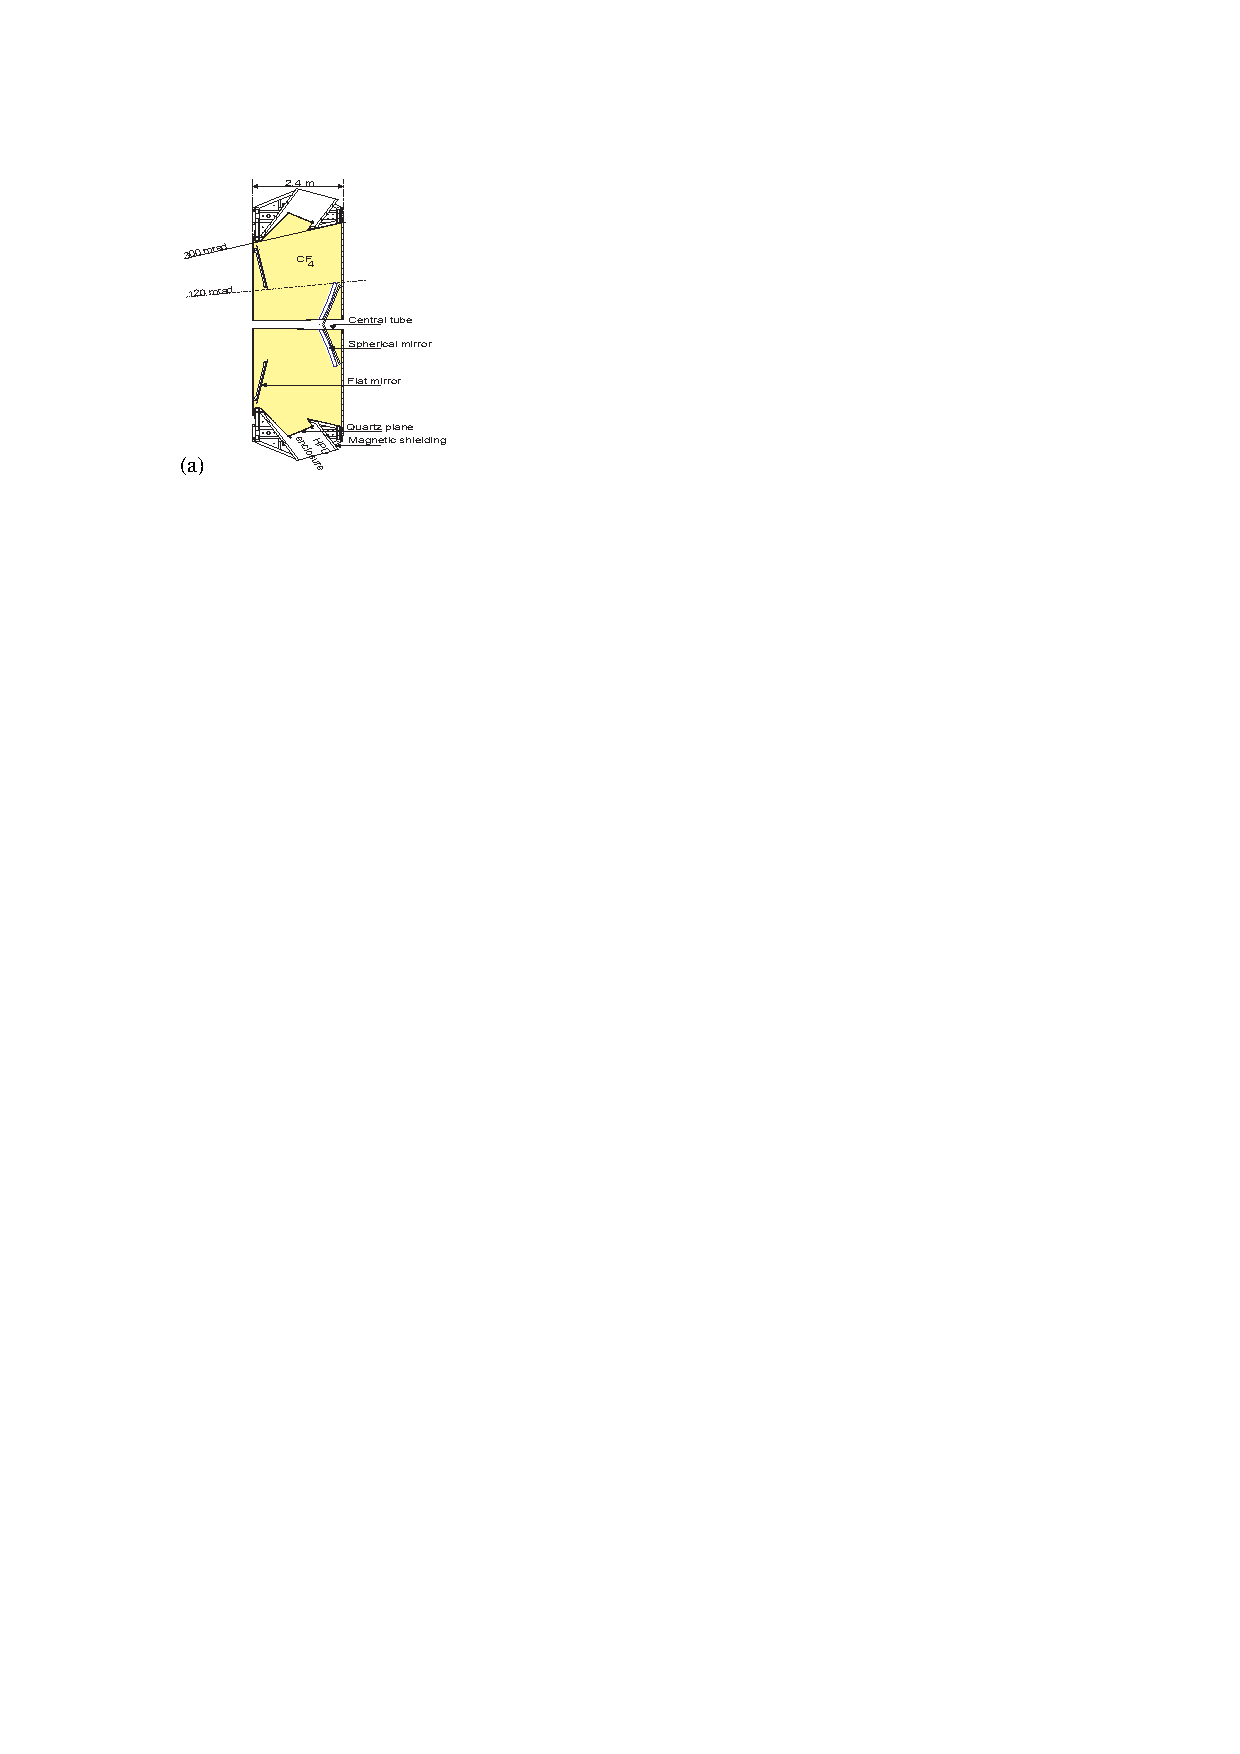
\includegraphics[width=1.0\textwidth]{figs/Detector/richtwo_layout.pdf}
        \caption{\richtwo}
    \end{subfigure}
    \caption{Schematic the \richone and \richtwo sub-detectors from Ref.~\cite{Alves:2008zz}.}

    \label{fig:Dec_rich_layout}   
\end{figure}
%%%%%%%%%%%%%%%%%%%%%%%%%%%%%%%%%%%%%%%%%%%%%%%%%%%%%%%%%%

\subsubsection{\richone}

{\color{Red}
\begin{itemize}
\item radiator and refractive indices 
\item talk about aero gel being removed
\item find some references 
\end{itemize}
}

\subsubsection{\richtwo}

{\color{Red}
\begin{itemize}
\item radiator and refractive indices 
\end{itemize}
}

\subsection{Calorimeters}

The calorimeters measure the energy deposited by particles. This is crucial for the reconstruction of neutral particles that don't leave tracks in the tracking stations. Additionally, the calorimeter plays an important role in the triggering of events.

\subsubsection{Pre-shower detector}
\subsubsection{Electronic Calorimeter}
\subsubsection{Hadron calorimeter}

\subsection{Muon system}

%%%%%%%%%%%%%%%%%%%%%%%%%%%%%%%%%%%%%%%%%%%%%%%%%%%%%%%%%%
\begin{figure}[!h]
    \centering
    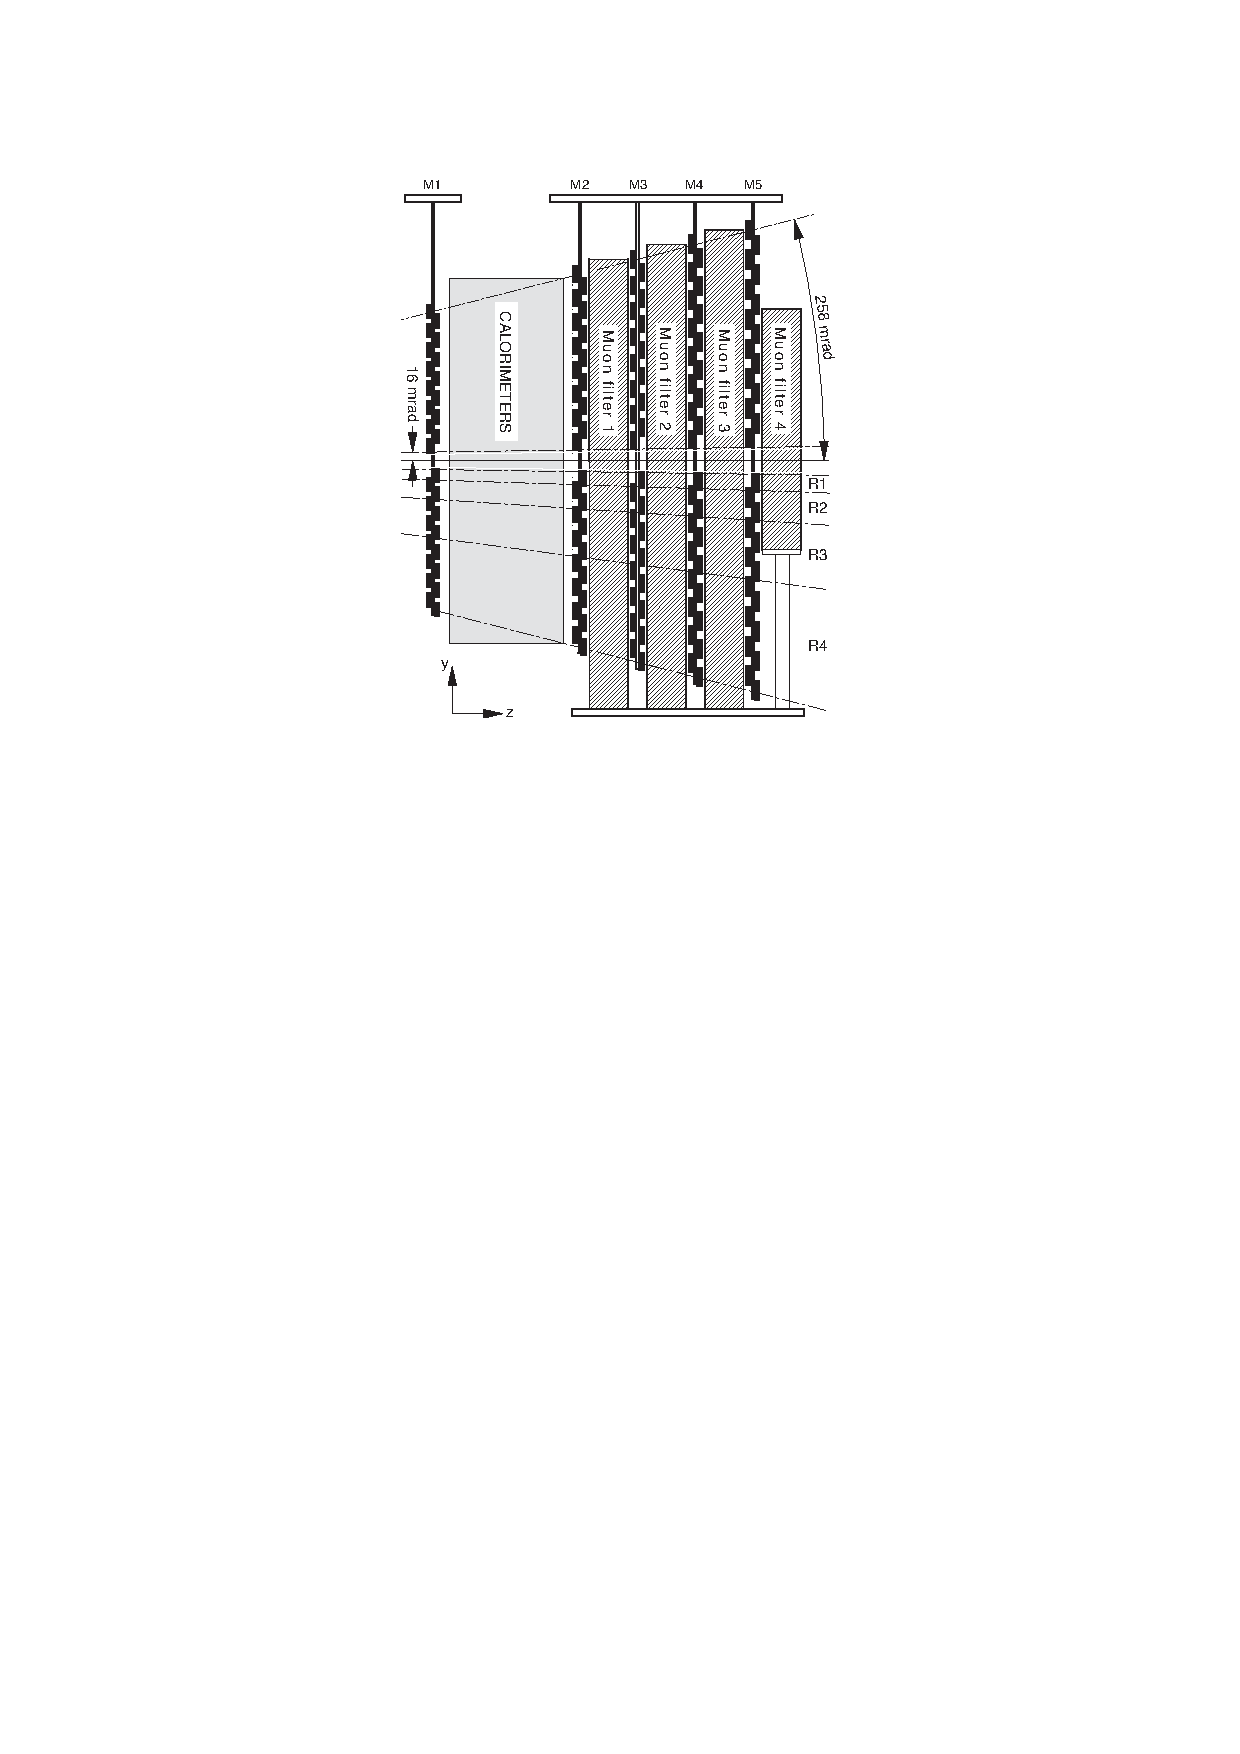
\includegraphics[width=0.4\textwidth]{figs/Detector/muon_layout.pdf}
    \caption{Schematic of the Muon sub-detector, from Ref.~\cite{Alves:2008zz}.}
    \label{fig:Dec_muon_schematic}   
\end{figure}
%%%%%%%%%%%%%%%%%%%%%%%%%%%%%%%%%%%%%%%%%%%%%%%%%%%%%%%%%%

\subsection{Trigger}
\subsubsection{\lone}
\subsubsection{\hltone}
\subsubsection{\hlttwo}

\subsection{Reconstruction}
\subsubsection{Track Reconstruction}


%%%%%%%%%%%%%%%%%%%%%%%%%%%%%%%%%%%%%%%%%%%%%%%%%%%%%%%%%%
\begin{figure}[!h]
    \centering
    \begin{subfigure}[t]{0.4\textwidth}
        \centering
        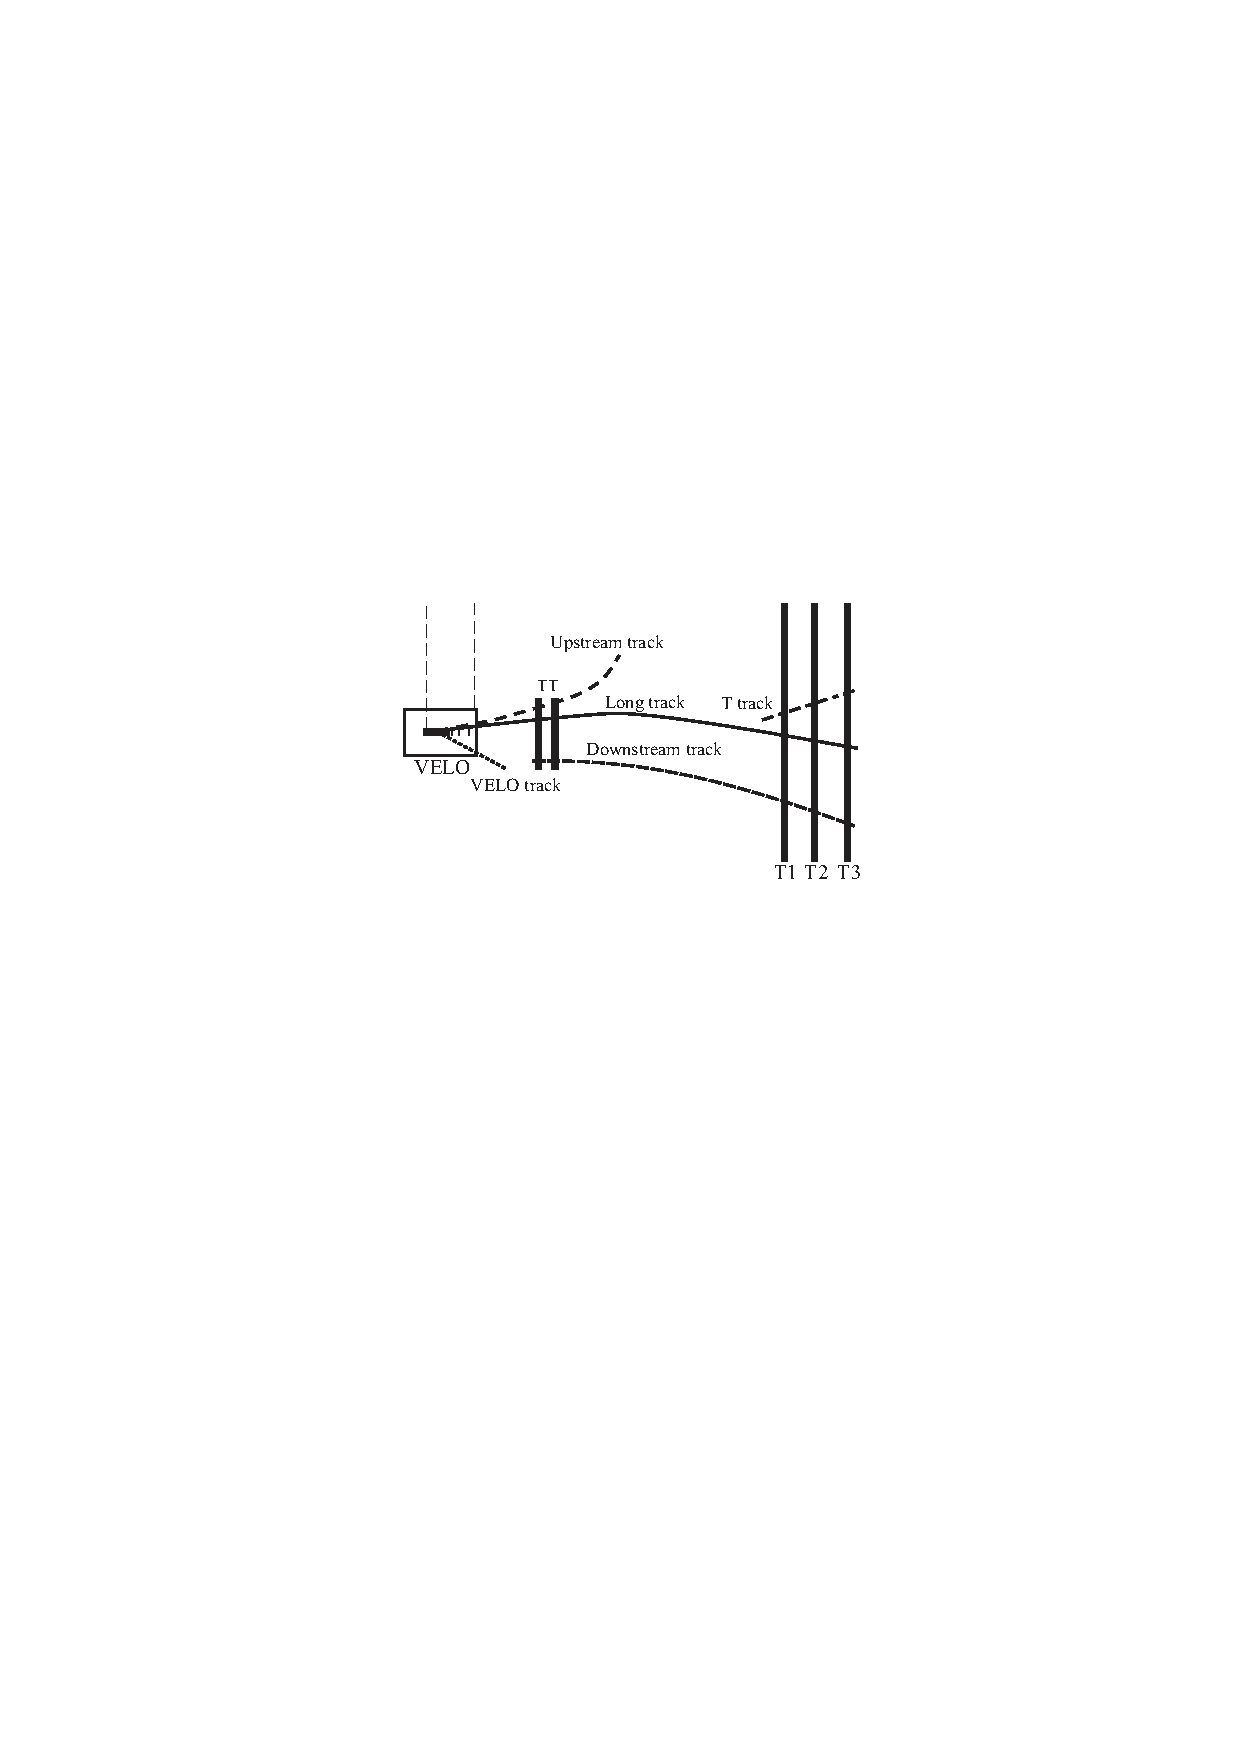
\includegraphics[width=1.0\textwidth]{figs/Detector/reco_track_types.pdf}
    \end{subfigure}
    \begin{subfigure}[t]{0.4\textwidth}
        \centering
        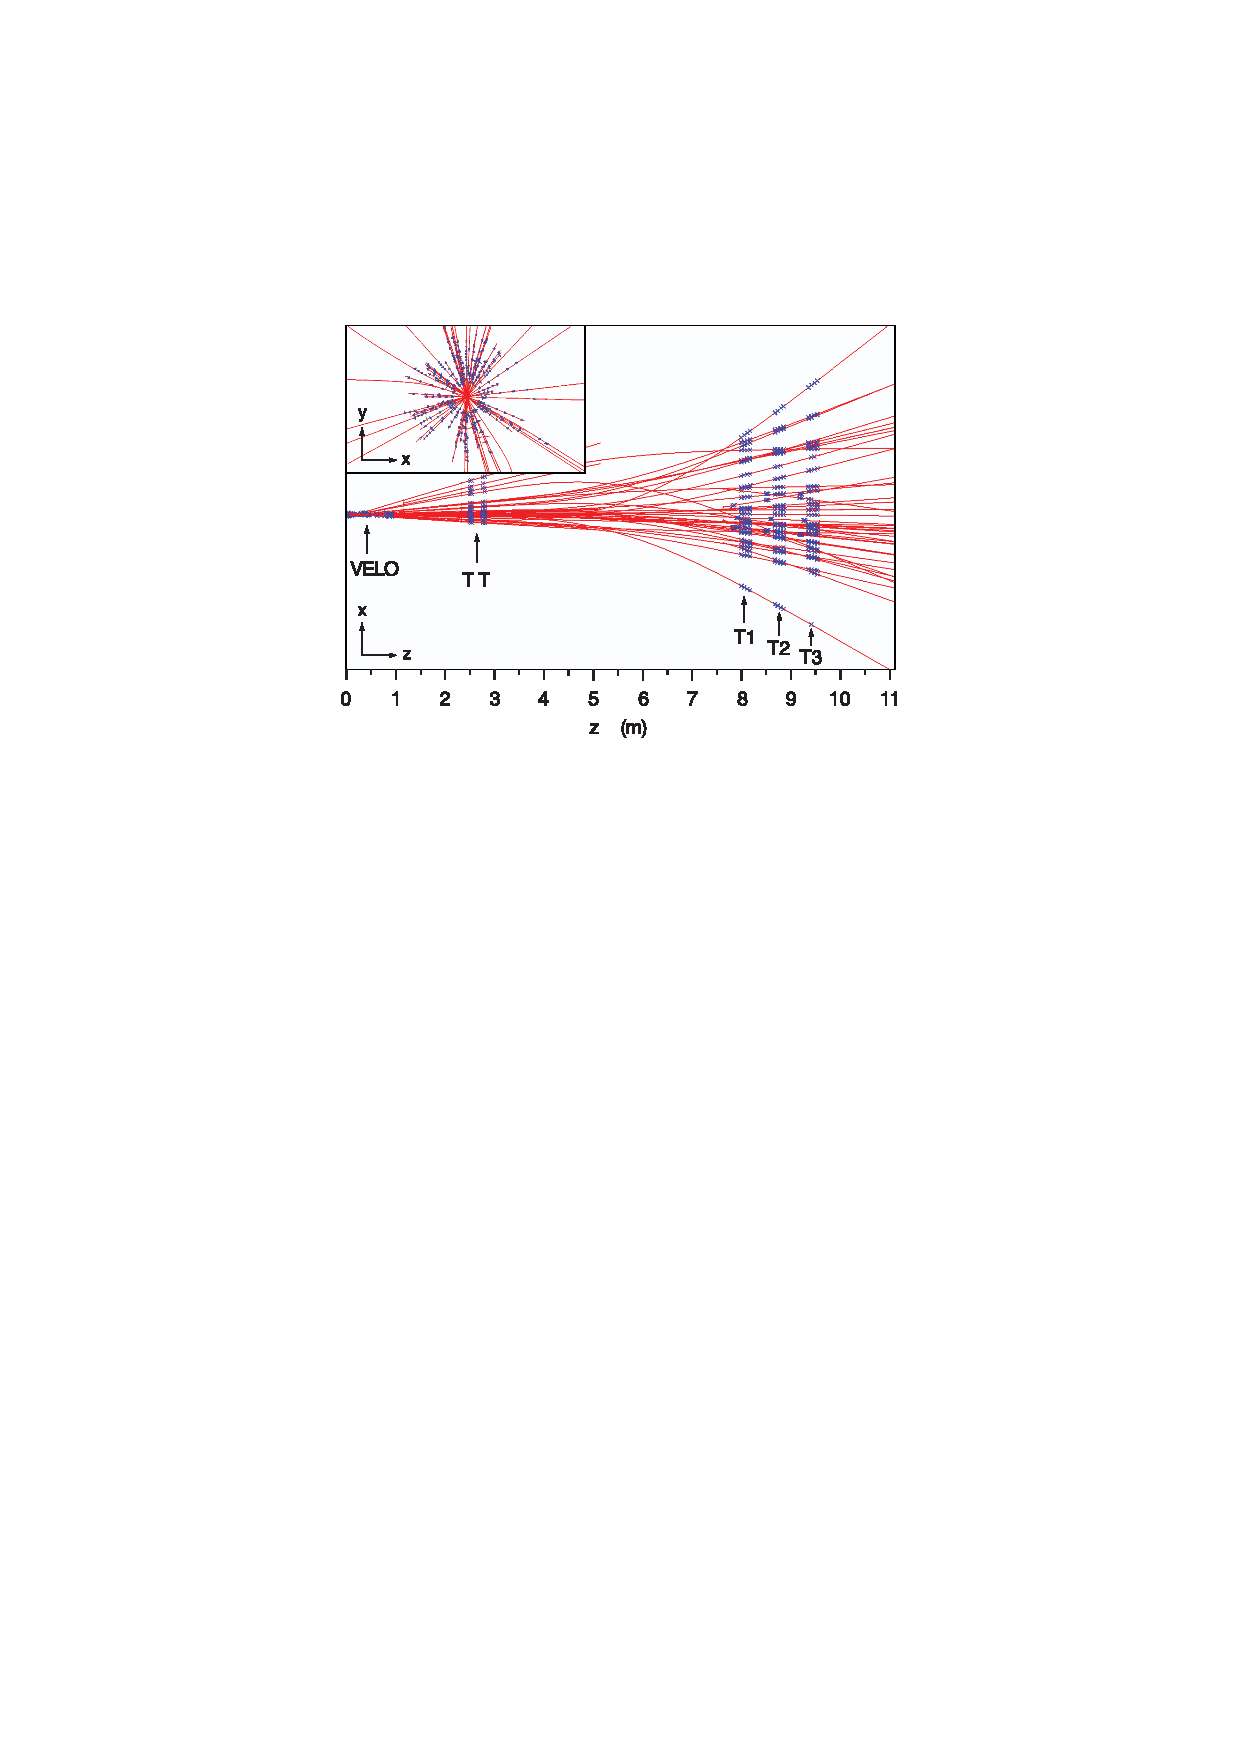
\includegraphics[width=1.0\textwidth]{figs/Detector/reco_track_reco.pdf}
    \end{subfigure}
    \caption{Diagram of the different track reconstruction types (left) and an illustration of the reconstructed tracks in a typical event from Ref.~\cite{LHCb-DP-2014-002}.}
    \label{fig:Dec_reco_tracks}   
\end{figure}
%%%%%%%%%%%%%%%%%%%%%%%%%%%%%%%%%%%%%%%%%%%%%%%%%%%%%%%%%%

\section{VELO resolution and luminosity determination}